% Cap�tulo 3
\chapter{Desenvolvimento}

\section{Definição da ideia}

A ideia do sistema originou-se da necessidade observada dentro do curso de TADS, onde uma parte dos alunos não conseguiam se expressar bem na língua inglesa, seja através da fala ou escrita. Isso acontecia até mesmo com aqueles que entendiam bem na leitura e/ou escuta. Essa é uma realidade no que diz respeito ao estudo de línguas no âmbito de faculdades e escolas, e podem ocorrer por diversos motivos. Segundo Paul Wilson, um estudioso de línguas da Faculdade de Filosofia e Línguas, que realizou estudos em diversas salas de aulas na Polônia, “Os alunos que estão em sala de aula possuem um bloqueio quando falam, em outra língua e em público, pois possuem medo de errar e que seus colegas o zombem. Logo, a vergonha tem grande influência negativa no processo de aprendizagem” \citeonline{Wilson}. Isso se reflete na realidade do curso de TADS, pois a leitura e a escuta, que teoricamente são habilidades que podem ser desenvolvidas sozinhas, são uma das primeiras a serem adquiridas.

Essas pessoas podem ser classificadas no nível intermediário, e avançar nos estudos nessas condições se mostra complicado, por vezes. Isso acontece pelo problema de Platô (ou efeito Platô). Nele, o estudante em questão sente que não evolui tanto após alcançar um certo ponto, o que acaba por frustrá-lo e desmotiva a continuar avançando nos estudos. Isso ocorre porque ao começar a aprender alguma coisa, é mais fácil absorve informações e fazer ligações entre esses conhecimentos adquiridos, sendo assim a sensação de estar aprendendo mais rápido é maior em relação a quando se possui uma quantidade de conteúdo mais avançado, onde poucas coisas são realmente novas ou simples \citeonline{Thomas}. 

Visto isso, foi pensando também em adaptar a ideia principal para ajudar os alunos de línguas a conseguir ultrapassar essa barreira desmotivadora. Uma forma genérica levada em consideração, foi a hipótese imposta por Malcolm Gladwell, no seu livro Fora de Série – Outliers \citeonline{Gladwell}. Nesta obra é afirmado que são necessárias dez mil horas (aproximadamente dez anos) para executar uma tarefa com excelência. No entanto, é deixado claro que a repetição, realizada por si só e de qualquer forma, não é a essencial, e sim aquela consciente, sempre procurando fazer com foco e da melhor forma. Está é uma ideia ampla e que foi tomado no contexto de estudo de línguas, onde a repetição é uma ótima forma de aprender, mesmo que não leve a perfeição.

\section{Validação da ideia}

Com uma problemática identificada e uma proposta de solução, foi iniciada uma pesquisa para averiguar a utilidade e a didática adequada para um sistema que auxiliasse esse perfil de estudante. Primeiramente, foi feito uma sondagem com os professores da \abrv[DIATINF -- Diretoria Acadêmica de Gestão e Tecnologia da Informação]{DIATINF} que ajudaram a amadurecer mais a ideia, fazendo assim que a problemática fosse vista sob novas óticas. Depois foi feita a validação junto aos possíveis usuários finais: alunos do IFRN. Para isso, além de uma conversa com alunos de TADS, foi criado um questionário para colher opiniões em relação às funcionalidades propostas. O questionário foi divulgado nos grupos do IFRN (DIATINF e Spotted 2.0) e na \abrv[UFRN -- Universidade Federal do Rio Grande do Norte]{UFRN} (no grupo de bacharelado em tecnologia da informação). Foram obtidas 71 respostas, no período de um mês. O resultado de algumas perguntas pode ser observado a seguir:

\begin{figure}[htb]
	\centering
  	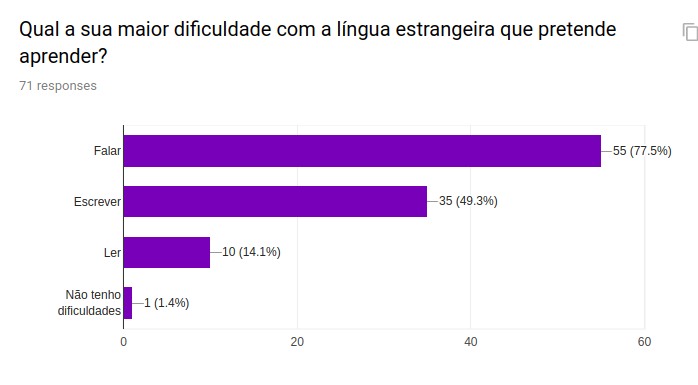
\includegraphics[scale=0.55]{src/imagens/graf1.png}
  	\textsf{\caption{Resultado da pesquisar referente a maior dificuldade dos estudantes entrevistados ao estudar uma língua estrangeira}}
  	\label{fig:FiguraTeste}
\end{figure}

\newpage

\begin{figure}[htb]
	\centering
  	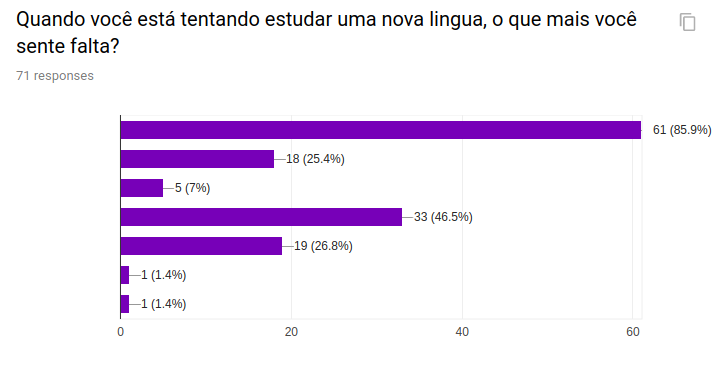
\includegraphics[scale=0.55]{src/imagens/graf2.png}
  	\textsf{\caption{Uma outra pessoa para praticar (85.9\%), confiança para falar outra língua na presença de outra(s) pessoa(s) (46.5\%), gramática (26.8\%)}}
  	\label{fig:FiguraTeste}
\end{figure}

Com essas duas perguntas direcionadas, foi possível validar as funcionalidades de criação de salas de conversas, uma vez que a maior dificuldade constatada é a fala e a confiança ao se expressar em público. Com as salas virtuais, é possível que estes problemas sejam amenizados, uma vez que o usuário não estaria na frente de ninguém, apenas de um dispositivo conectado à internet, conversando com outras pessoas.

\begin{figure}[!ht]
	\centering
  	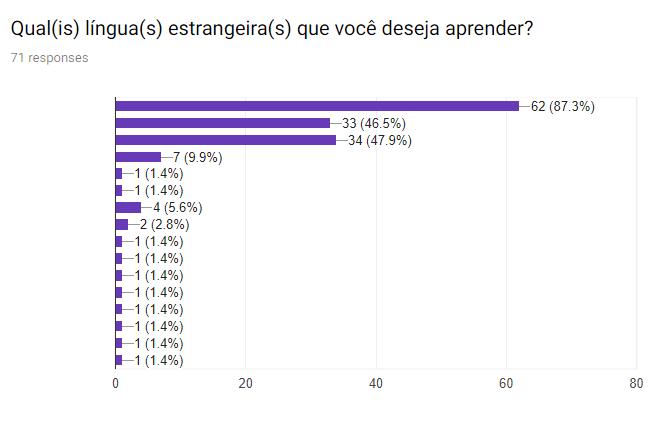
\includegraphics[scale=0.60]{src/imagens/graf3.png}
  	\textsf{\caption{Inglês (87.3\%), francês (47.9\%), espanhol (46.5\%)}}
  	\label{fig:FiguraTeste}
\end{figure}

Analisando as respostas do questionário foi possível direcionar quais são as línguas de mais frequentemente estudadas pelos possíveis usuários do sistema. Com essas informações foi possível se orientar e delimitar quais línguas seriam abordadas dentro do sistema, além do Português. Seria inviável começar com muitos idiomas, pois o trabalho para dar suporte ao sistema a mais um idioma é relativamente grande, pois é preciso traduzir cada texto, em cada página, como vai ser explicado mais adiante. Esse foi mais um motivo para ter criado essa pergunta. 

É importante ressaltar que embora o BNativus tenha o  intuito inicial de ajudar os brasileiros, ele está estruturado visando uma futura escalabilidade em nível internacional. Por isso, foi criado um pequeno questionário direcionado a estrangeiros. Apesar de ter sido divulgado em fóruns estrangeiros, não houve um \textit{feedback} considerável para ser incluído no conjunto no escopo das funcionalidades definidas. Futuramente ele pode ser adaptado e utilizado novamente, com o intuito de conhecer melhor os estrangeiros que utilizam ou pretendem utilizar o sistema.

\section{Escolha das tecnologias}

Com a evolução da WEB, a construção de sistemas web cresceu em grande escala, junto com a sua complexidade. E para suprir as necessidades que surgiram, inúmeras tecnologias foram sendo desenvolvidas como frameworks, web services, soluções em nuvem (computação em nuvem), entre outros. Diversos conceitos foram surgindo e evoluindo ao mesmo ritmo, conceitos esses que ajudam aos sistemas a se tornarem cada vez mais robustos, escaláveis, orientando aos profissionais da área a melhor forma de entregar o produto, com o máximo de valor aos usuários. Como exemplos há os processos de software (scrum, xp e etc), testes (unitários, aceitação, stress e etc.) e UX (\textit{user experience}). 

É fato que a maioria dessas tecnologias procuram resolver problemas parecidos, o que acaba montando um mercado com ferramentas semelhantes em suas propostas e forma de funcionar. Diante de tantas opções, é importante escolher bem as tecnologias e práticas que serão utilizadas durante o desenvolvimento, e que melhor se encaixe as necessidades encontradas, deixando claro para a equipe, para que assim possa se seguir um padrão e mantenha-se a organização. 

Durante o curso de Análise e Desenvolvimento de Sistemas são estudadas em sala muitas dessas técnicas e tecnologias, sendo impostas as suas importâncias e onde seria a sua melhor aplicação. Há também as experiências adquiridas fora de ambiente, em eventos proporcionados pelo próprio IFRN e ainda o estágio, que é uma exigência para a conclusão do curso.

As tecnologias utilizadas para a construção do BNativus foram escolhidas baseadas nessas experiências citadas. Inicialmente foi escolhido o Scrum como processo de software, uma vez que ele se demonstrou eficiente ao longo do curso, onde foi utilizado em projetos pessoais, acadêmicos, e extra acadêmicos (no estágio, por exemplo), além de ser maleável para diferentes tipos de equipe, que no caso desse projeto é constituído por apenas uma pessoa. Logo após, foi definido o framework web Ruby on Rails para desenvolver o sistema em si. Levado em consideração também a experiência que já havia na equipe, pois ele foi bastante utilizado durante o curso, tanto dentro do âmbito escolar (no Projeto de Desenvolvimento de Software, ou PDS), quanto fora dele (em projeto pessoais e no estágio), na maioria dos casos se mostrando uma opção estável, com inúmeras bibliotecas construídas e mantidas pela comunidade (que mostra bem ativa), que auxiliaram durante o desenvolvimento.

Uma coisa que faz parte do desenvolvimento de qualquer sistema é a configuração do seu ambiente, ou seja, instalar e configurar todas as ferramentas necessárias para que seja possível executá-lo. E isso pode ser, por vezes, custoso ou problemático, porque se houver algum defeito na máquina que já estiver configurada, de modo que seja necessário formatá-la, toda configuração deve ser feitas novamente, e isso leva tempo, mesmo se houver algum tipo de documentação. No momento de colocar em produção é provável que seja um obstáculo, pois o mesmo ambiente deve ser replicado em algum servidor. Tendo isso em mente, foi definido, desde o início, o uso do Docker para que esses tipos de transtornos pudessem ser contornados.

O uso do DevOps e testes unitários, junto com o Docker, foi uma forma de forçar o uso desses conceitos na prática, uma vez que durante o curso eles foram amplamente difundidos, tanto dentro quanto fora de sala de aula, como conceitos importantes e bastante utilizados no mercado de trabalho, logo seria importante usá-los em algum momento e criar uma experiência básica em uma aplicação, com usuários e tempo de entrega reais. Esses conceitos citados deveriam ser abstraídos e implantados em serviços específicos da AWS.

\section{Construção do sistema}

A solução aqui apresentada foi idealizada em outubro de 2017, ou seja, antes do período 2018.1, que é quando deveria ser criado necessariamente o trabalho de conclusão de curso. Dessa forma houve mais tempo para validar, amadurecer e construir o BNativus, além da possibilidade de conciliar bem com estágios, trabalho e a faculdade, sem que houvesse uma sobrecarga.

Como a equipe é composta apenas por uma pessoa, foi necessário realizar uma adaptação do Scrum, e o simplificá-lo de modo que não foi necessário reuniões semanais ou encontros constantes com o cliente. Com isso, o desenvolvimento completo do sistema levou por volta de 3 meses, e esse período foi dividido em três sprints (uma por mês). Mesmo que não houvesse um contato direto com o cliente, e assim entregar um valor mais imediato para os usuários ao fim de cada sprint (valor), estabelecer essas etapas foi de suma importância para se auto policiar e se manter organizado com as entregas.

\subsection{Estabelecer sprints e requisitos}

Como já foi explicado, o processo de software scrum aqui utilizado foi adaptado às necessidades, e por isso não houve a necessidade de product owner, por exemplo. Todavia, a sua essência foi utilizada e o backlog foi criado com todos as tarefas e ideias necessárias para que o sistema se tornasse usual e suprisse a necessidade do usuário alvo. Para auxiliar a montagem do backlog, além de manter a orientação ao longo do desenvolvimento, enxergando melhor a solução, foi agregado ideias e gerados alguns artefatos \abrv[UML -- Unified Modeling Language]{UML}. 

A UML tornou-se a linguagem universalmente aceita para documentação de projetos de software. Ela pode ser definida também como uma linguagem visual usada para transmitir ideias de projeto. Dessa forma, padronizações de projeto de software são criados, permitindo descrever fragmentos de projeto e reusar ideias, ajudando desenvolvedores a se nivelar com experiências passadas ou transmiti-las para outros. Utilizar a UML aumenta as chances de se trabalhar em um sistema com maior análise, definindo melhor como resolver os problemas e também o que é preciso programar, além de criar um meio fácil de comunicar, revisar, implementar e evoluir o projeto \citeonline{Larman}.

Para representar essa linguagem visual, são utilizados de diagramas. Durante o curso de TADS, esses padrões e diagramas foram apresentados e criados na prática, com a geração de alguns artefatos para sistema desenvolvidos dentro das disciplinas. Como exemplo, podem ser citados diagrama de objetos, diagrama de componentes, diagrama de implementação e etc. Para o caso desse projeto, foi utilizado o caso de uso que tem como objetivo descrever um cenário que mostra as funcionalidades do sistema do ponto de vista do usuário \citeonline{Larman}. Mas antes de construí-lo, foram elencados os requisitos funcionais e não funcionais que são demonstrados a seguir:


\begin{table}[]
\centering
\caption{Listagem dos requisitos funcionais}
\label{my-label}
\begin{tabular}{|l|l|}
\hline
RF01 & Cadastro e gerenciamento de salas   \\ \hline
RF02 & Cadastro e gerenciamento de debates \\ \hline
RF03 & Cadastro e gerenciamento de artigos \\ \hline
RF04 & Votar em debate                     \\ \hline
RF05 & Votar em artigo                     \\ \hline
RF06 & Comentar debate                     \\ \hline
RF07 & Comentar artigo                     \\ \hline
RF08 & Autenticação do usuário             \\ \hline
RF09 & Editar perfil                       \\ \hline
RF10 & Compartilhar salas                  \\ \hline
RF11 & Compartilhar debates                \\ \hline
RF12 & Compartilhar artigos                \\ \hline
RF13 & Alterar idioma do sistema           \\ \hline
\end{tabular}
\end{table}

\begin{table}[]
\centering
\caption{Listagem dos requisitos não funcionais}
\label{my-label}
\begin{tabular}{|l|l|}
\hline
RNF01 & Autenticação com redes sociais \\ \hline
RNF02 & Segurança                      \\ \hline
\end{tabular}
\end{table}

Após esse passo, que foi possível graças às estratégias de validação, as funcionalidades mais críticas se tornaram mais claras e foi possível criar o diagrama de casos de uso e suas descrições para melhor entendimento do ator final do projeto. Este documento auxiliar explicitou se as funcionalidades apresentadas poderiam solucionar o problema. Abaixo, o diagrama de casos de uso:

\newpage

\begin{figure}[!htb]
	\centering
  	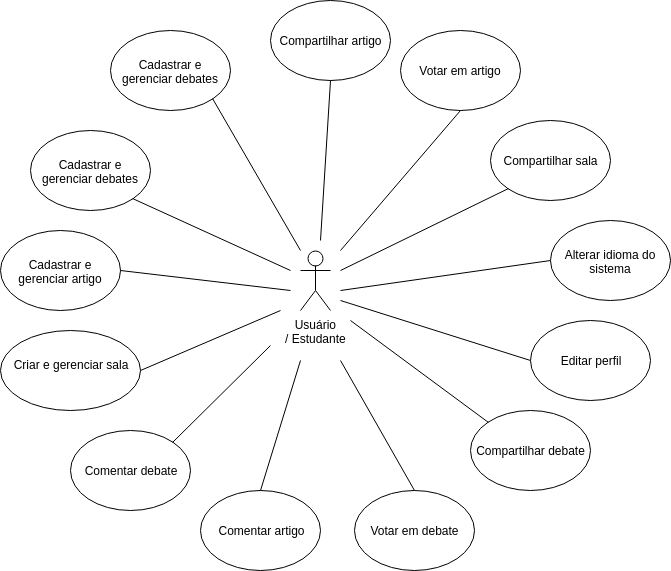
\includegraphics[scale=0.60]{src/imagens/CDU.png}
  	\textsf{\caption{Diagrama de caso de uso do BNativus}}
  	\label{fig:FiguraTeste}
\end{figure}

Como pode ser observado na figura acima o autor principal, que é o estudante, tem acesso a todos os recursos do sistema a partir do momento em que ele está autenticado. No futuro poderá haver a necessidade de outros autores, como um administrador, mas para as necessidades atuais, não se fez necessário um controle mais a fundo do conteúdo gerado, uma vez que o sistema será alimentado pelos próprios usuários. 

\subsection{Fluxo de organização}

Após definir o problema, validar a solução, delimitar o escopo, criar artefatos para auxiliar no entendimento do sistema, foi iniciado o desenvolvimento do sistema de fato. É válido ressaltar que, mesmo havendo apenas uma pessoa na equipe foi necessário o uso de alguma ferramenta para controlar e orientar as sprints definidas, organizar novas ideias que surgiram durante a construção, tal como \textit{bugs}, armazenar a documentação, anotações e sugestões. Hoje existem diversas ferramentas que suprem essas necessidade. No projeto foi escolhido o Trello, por sua versatilidade e praticidade no que diz respeito à organização de projetos.
	
A sua interface simples e intuitiva é organizada em \textit{boards}, e nelas existem várias colunas de listas, todas dispostas horizontalmente, e nessas colunas residem os chamados \textit{cards}, que são cartões com tópicos específicos (sendo possível criar lista de tarefas, adicionar arquivos, realizar comentários e etc). Na figura 6 é mostrado o \textit{board} do BNativus:

\begin{figure}[!htb]
	\centering
  	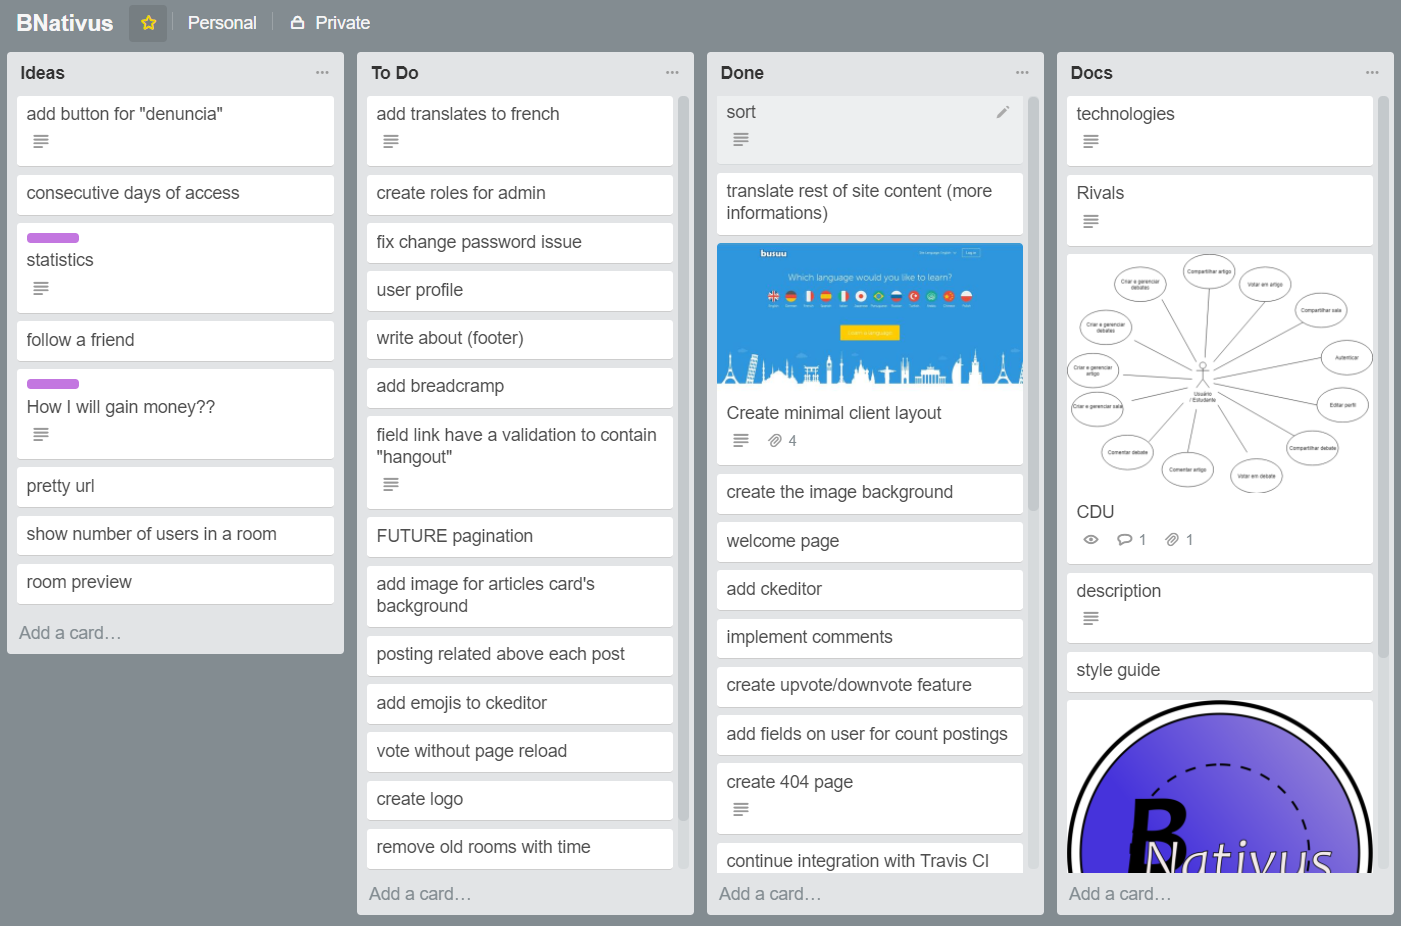
\includegraphics[width=16cm, height=10cm]{src/imagens/trello.PNG}
  	\textsf{\caption{\textit{Boards} do Trello construidos durante o desenvolvimento}}
  	\label{fig:FiguraTeste}
\end{figure}

Como pode-se observar, o desenvolvimento seguiu quatro listas, que seguiam o fluxo partindo da esquerda, para a direita:

\begin{enumerate}
   \item Ideias: Nelas foram colocadas ideais que foram surgindo durante o desenvolvimento, ideais essas que partiram da própria equipe, de professores e colegas que acompanharam o projeto e do orientador.
   \item To Do: São melhorias as tarefas que ficaram para se fazer no futuro. Não são imprescindíveis para o funcionamento do projeto, mas seriam importantes de serem implementadas.
   \item Done: Mantém todas tarefas que foram concluídas.
   \item Docs: Armazena artefatos que foram gerados durante todo o desenvolvimento, desde os formulários usados na fase de concepção até senhas de arquivos de terceiros utilizados
 \end{enumerate}
 
 \section{Iniciado o Desenvolvimento}
 
 \subsection{Configurando o ambiente}
 
Como já foi explicado anteriormente, para montar o ambiente da aplicação foi usado o Docker. Mais precisamente o docker-compose, pois foram necessários dois contêineres, um para a aplicação web em si e outro para o banco de dados. Para começar a utilizar o docker-compose, é preciso basicamente seguir três passos. A seguir, será explicado melhor como isso foi feito:

\begin{enumerate}
       \item Criar o arquivo Dockerfile, que é responsável por definir e reproduzir o ambiente do projeto em qualquer lugar, e colocá-lo na raiz no projeto. Na figura 7 temos, o Dockerfile que foi criado para a aplicação em questão.

        \begin{figure}[!htb]
        	\centering
          	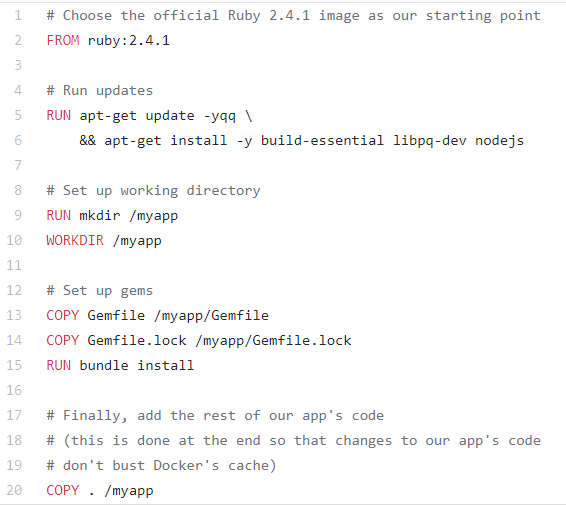
\includegraphics[width=12cm, height=10cm]{src/imagens/dockerfile.PNG}
          	\textsf{\caption{Dockerfile utilizado durante o desenvolvimento}}
          	\label{fig:FiguraTeste}
        \end{figure}

       \item Configurar os serviços que vão constituir a aplicação no arquivo docker-compose.yml, para que assim seja possível executá-los de forma conjunta em um ambiente isolado. Como ele foi estruturado na aplicação em questão.
       
       \newpage
       
       \begin{figure}[!htb]
        	\centering
          	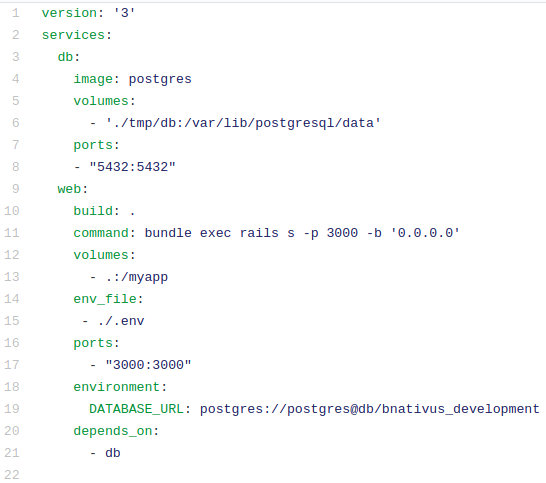
\includegraphics[width=12cm, height=10cm]{src/imagens/docker-compose.png}
          	\textsf{\caption{Docker-compose utilizado durante o desenvolvimento}}
          	\label{fig:FiguraTeste}
        \end{figure}
        
        \item Executa o comando docker-compose up web db para executar a aplicação, utilizando esses dois arquivos.
\end{enumerate}

A figura 8 mostra um arquivo de configuração docker-compose.yml baseado na linguagem YAML, utilizado comumente para configurações por sua facilidade de leitura a humanos. Através da indentação, é possível observar que são utilizados dois serviços necessários para a aplicação ser executada corretamente:

\begin{enumerate}
    \item Db: reservado para configurar as informações relacionadas ao banco de dados, como por exemplo a imagem que vai ser utilizada para montar o container, o volume, que pode ser utilizado em múltiplos serviços, e o mapeamento da porta de acesso;
    \item Web: Mapeia as informações do sistema em si, executando o servidor, mapeando a porta e etc.
\end{enumerate}

O banco de dados é um conceito fundamental a ser destacado. Quando se trata de construir um sistema web é primordial que os dados gerados pelos usuários sejam armazenados, formando uma coleção de dados. De posse dessas informações, operações podem ser realizadas posteriormente, como consultas, modificações e exclusões. É por isso que o container web depende do container db para funcionar corretamente. Existem diversos tipos de bancos, com os mais diversos padrões para diferentes tipos de casos.

Banco de dados do tipo relacional são bastante comuns e largamente utilizados em sistemas web. Os recursos principais são abstraídos em forma de tabela, que se relacionam. Existem diversos banco de dados que englobam esse conceito como o MySQL e SQL Server. O BNativus utiliza o PostgreSQL, um banco de dados de código aberto largamente usado pela comunidade. A figura 9 demonstrado um diagrama com as tabelas utilizadas no sistema:

\begin{figure}[!htb]
	\centering
  	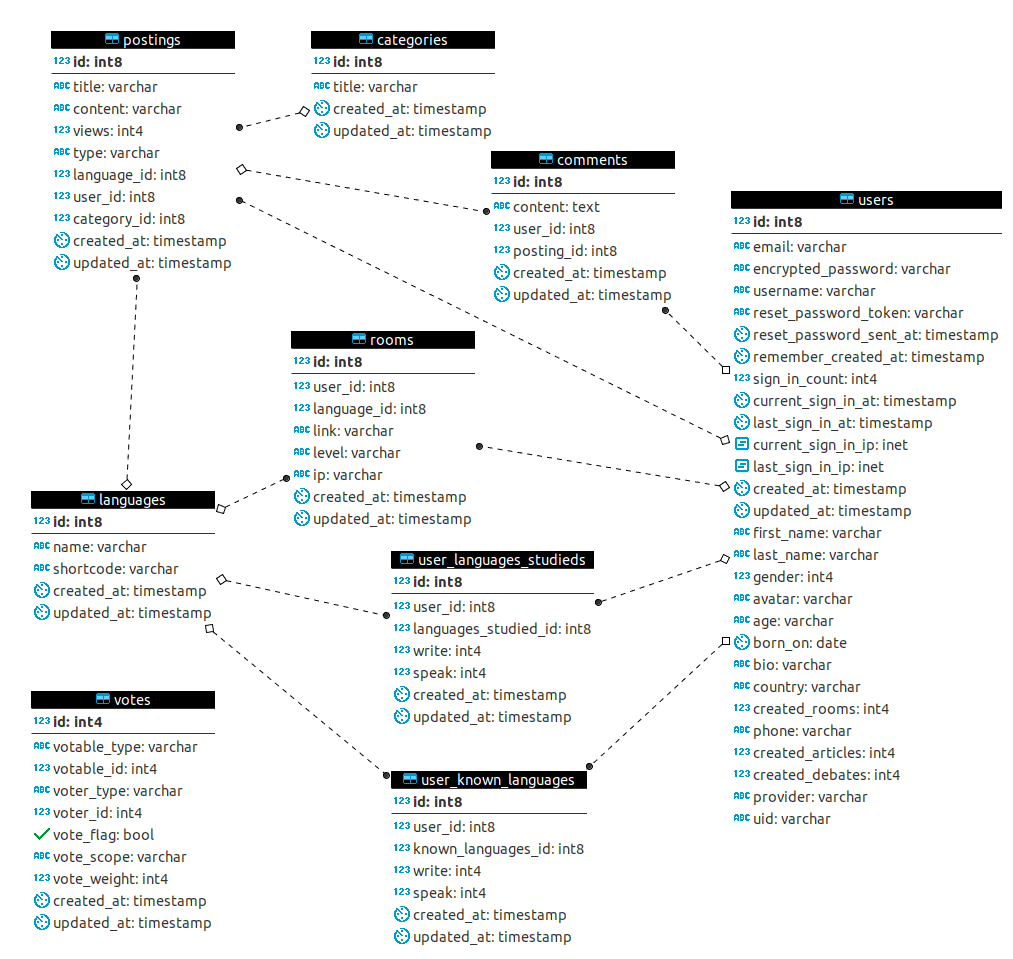
\includegraphics[width=16cm, height=14cm]{src/imagens/diagram_db_bnativus.png}
  	\textsf{\caption{Diagrama de banco de dados da aplicação}}
  	\label{fig:FiguraTeste}
\end{figure}

\subsection{Construção do MVP}

Seguindo os conceitos já apresentados de MVP e Scrum, nesta seção serão apresentados as três sprints estabelecidas, junto com os resultados de cada uma delas. Vale ressaltar que no scrum as sprints possuem durações menores, com dias ou semanais. No entanto, como o desenvolvimento foi realizado por apenas uma pessoa, foi preciso realizar simplificações, para conciliar com o curso de \abrv[TADS -- Tecnólogo em Análise e Desenvolvimento de Sistemas]{TADS} e o estágio, que estava vigente na fase de desenvolvimento.

\subsubsection{Primeira sprint}

Foram criados alguns casos de uso, como foi explicitado na figura 5, e cada um deles foram implementados ao longo do desenvolvimento do projeto. A ordem de implementação seguiu a ideia de requisitos mais críticos ao sistema primeiro, ou seja, aqueles que são essenciais para o funcionamento pleno do software, solucionando a problemática maior. A seguir, serão revelados cada um deles.

 \begin{enumerate}[(i)]
   \item Cadastro e gerenciamento de salas
   
    O maior diferencial planejado	 para o projeto é a oportunidade de qualquer pessoa possa, de forma gratuita, se comunicar com outras através de áudio e vídeo, compartilhando assim os estudos e criando novas conexões. Todavia, logo foi notado que implementar uma funcionalidade como essa totalmente do zero seria inviável, pois exigiria um conhecimento a mais, o que iria implicar em maior tempo estudando, além de custos adicionais para manter estável e em produção. Portanto, foi decidido terceirizar essa parte do software para outro, que já está no mercado a mais tempo e se mostram mais confiáveis.

    Primeiro, foi estudado a possibilidade de usar o Skype\footnote{https://web.skype.com/}, serviço da Microsoft a mais tempo no mercado e mundialmente conhecido. Além de disponibilizar todas as funcionalidades exigidas gratuitamente, ainda possui clientes estáveis (software que necessitam ser baixados e instalados em algum computador ou smartphone), contudo, a plataforma web ainda estava em beta no momento de concepção do BNativus e demonstrava alguns \textit{bugs}, dentre outros problemas. Um lado positivo é que ele suporta 24 pessoas em uma única chamada. Mesmo assim, não coube às necessidades do sistema aqui apresentado. 
    
    Outro serviço no ramo das vídeo-chamadas que foi analisado foi o Temasys\footnote{https://temasys.io/}. Ele é baseado no protocolo de código aberto WebRTC (Web Real-time Communications), que segue o princípio da comunicação direta entre navegadores na arquitetura peer-to-peer\footnote{arquitetura de redes de computadores onde cada um dos pontos ou nós da rede funciona tanto como cliente quanto como servidor, permitindo compartilhamentos de serviços e dados sem a necessidade de um servidor central (https://pt.wikipedia.org/wiki/Peer-to-peer)}. Ele se parece estável e de fácil integração, utilizando apenas javascript, mas o que impediu a sua aplicação no BNativus foi o fato de ser pago, apesar de sua versão grátis durar apenas 30 dias.
    
    Seguiu-se a análise de outros serviços. Dentre os estudados, o que melhor se encaixou as necessidades foi Google Hangout. Criado em 2013, ele é totalmente gratuito com uma interface web (tal como o aplicativo) mais atraente e intuitiva, demonstrando estabilidade durante suas conexões de vídeo chamada. No momento do desenvolvimento deste artigo, ele permite dez pessoas por chamada, o que para um sistema que está apenas começando como o BNativus, foi julgado suficiente. 
    
    Logo após, foi pesquisado uma forma de integrar o Hangout a aplicação. Mas logo foi observado um empecilho, pois a API foi descontinuada em 25 de abril de 2017 por motivos de negócios da Google. Por isso, foi necessário procurar maneiras alternativas de agregá-lo ao sistema. A melhor forma foi criar um pequeno tutorial para os usuários, que não estão adaptados ao Hangout, pudessem criar salas no serviço externo e relacioná-las dentro do BNativus. As figuras X-Y mostram algumas capturas de telas de como criar uma sala de aula:

    \newpage
    
    \begin{figure}[!htb]
    	\centering
      	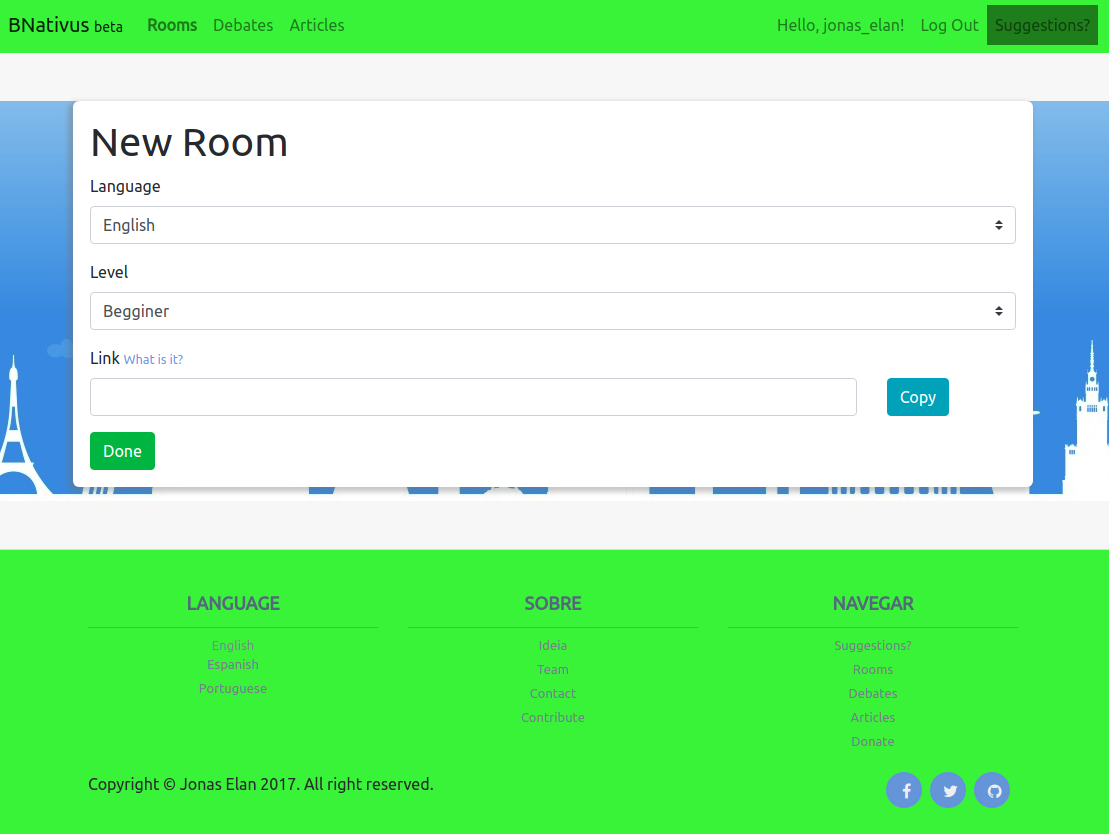
\includegraphics[scale=0.355]{src/imagens/criar-sala.png}
      	\textsf{\caption{Tela de criação de novas salas de conversa}}
      	\label{fig:FiguraTeste}
    \end{figure}
    
    \begin{figure}[!htb]
    	\centering
      	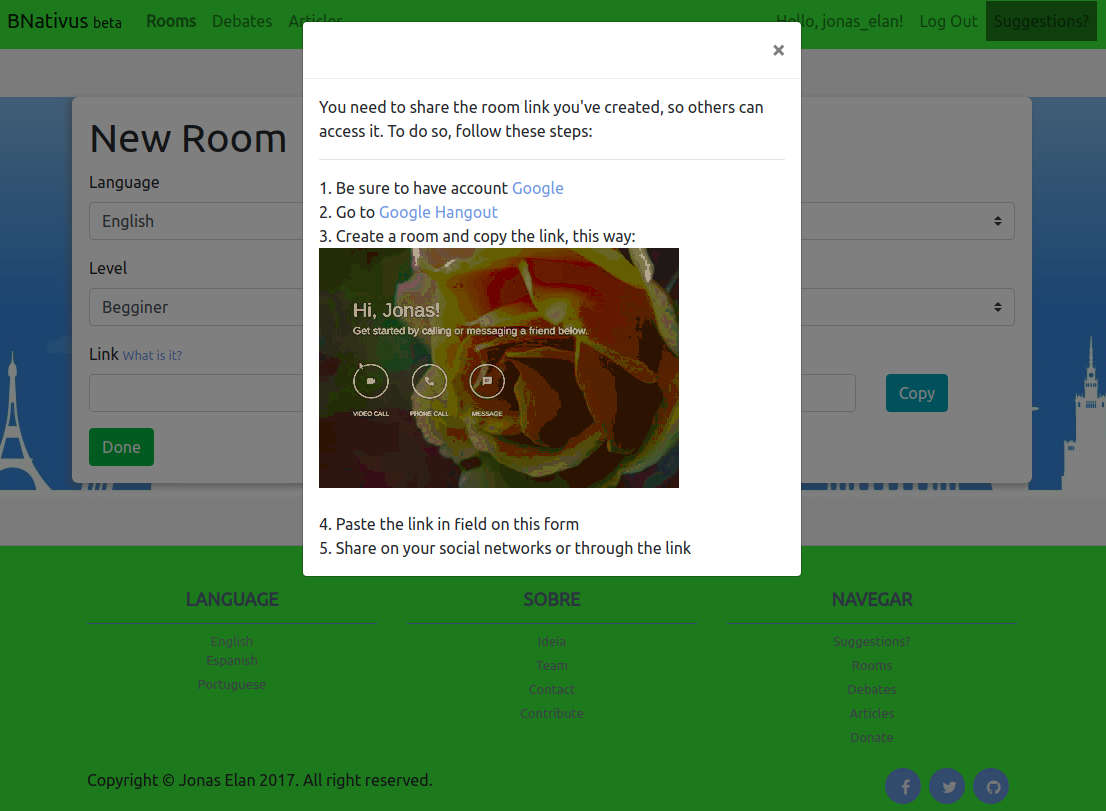
\includegraphics[scale=0.355]{src/imagens/criar-sala-tutorial.png}
      	\textsf{\caption{Representação do tutorial, localizado no modal, de criação de sala junto com o Hangout}}
      	\label{fig:FiguraTeste}
    \end{figure}
  
    Na figura 10 é apresentando o formulário com os campos necessários para criar uma sala. Os únicos campos necessários são a linguagem, o nível de fluência e o link da sala no Hangout. A forma de obter esse link é mostrada no modal que está representado na figura 11. Para tornar o processo mais intuitivo ainda, principalmente para aqueles que nunca usaram o serviço da Google em questão, é exposto um passo-a-passo, junto com um gif simples, explicando como abrir o Hangout, criar uma sala, gerar o link, copiar e colar na plataforma. Esse modal é apresentado após clicar no botão de ajuda, ao lado do campo “Link”.

   \item Cadastro e gerenciamento de debates e artigos
   
    Debates e artigos são dois recursos diferentes dentro da aplicação, no entanto são bastante semelhantes. É por isso que ao longo deste, e dos próximos tópicos, eles serão explicados na mesma seção e quando houver algum detalhe mais importante que os diferencie, será explicitado. Parte dessa semelhança ocorre porque ambos foram adicionados na aplicação com o mesmo objetivo principal, que é praticar a escrita na língua de estudo.

    Essa paridade de funcionalidade foi percebida logo no início do desenvolvimento, por isso foi utilizado a ideia de hereditariedade, tanto nos modelos quanto nos controladores de debates e artigos. Com isso, foi possível escrever o código apenas uma vez, e ser reaproveitamento pelos dois recursos.
    
    \begin{figure}[!htb]
    	\centering
      	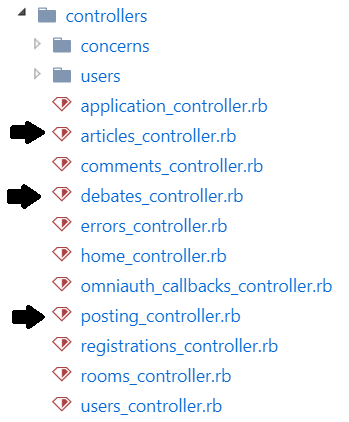
\includegraphics[scale=0.7]{src/imagens/Capturar.PNG}
      	\textsf{\caption{Controladores de dados usados no BNativus}}
      	\label{fig:FiguraTeste}
    \end{figure}
    
    \newpage
    
    \begin{figure}[!htb]
    	\centering
      	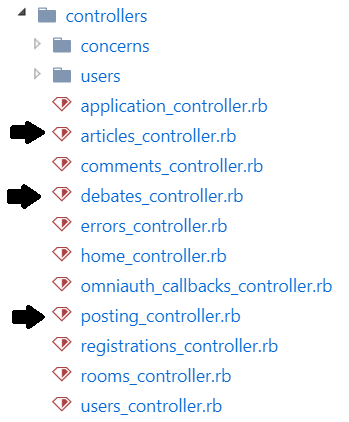
\includegraphics[scale=0.7]{src/imagens/Capturar.PNG}
      	\textsf{\caption{Modelos de dados usados no BNativus}}
      	\label{fig:FiguraTeste}
    \end{figure}
    
    Como pode-se observar nas figuras 12 e 13, foram criados o modelo Post (postagens) e o controlador Posting. Ele é o pai de debate e artigo, ou seja, todo o código escrito neles são comuns aos seus filhos. No caso em questão, foi inserido no controlador e modelo de postagem informações de conexões com outros modelos, validações de campos e a lógica de autenticação.

	Por padrão, o Rails segue o padrão Restful nas suas rotas (com flexibilidade para criar rotas personalizadas), o que reflete na forma como as ações dos controladores são estruturados. Por exemplo, quando se renderiza a tela com o formulário de criação de algum modelo, se passar pela ação new, e ao clicar no botão de submissão (realiza um POST), a ação create é chamada, que por sua vez está responsável pela criação. Da mesma forma acontece quando se deseja atualizar algo, onde se passa pela ação edit, para mostrar o formulário com as informações previamente cadastradas, e ao enviar os dados (através de um PUT), a ação update é chamada, atualizando o recurso. O framework Ruby ainda facilita essa renderização, pois relaciona o nome de cada uma dessas ações com os nomes das views. Por isso foi necessário separar as páginas em pastas diferentes, não utilizando necessariamente a mesma ideia de hereditariedade proposta nas outras camadas do sistema. Além do mais, foi pensando mais adiante, onde seria acrescentado novas funcionalidades a artigos, que não existiram em debates, e provavelmente utilizar a mesma view para trabalhar com as duas, não seria viável.

    
    \begin{figure}[!htb]
    	\centering
      	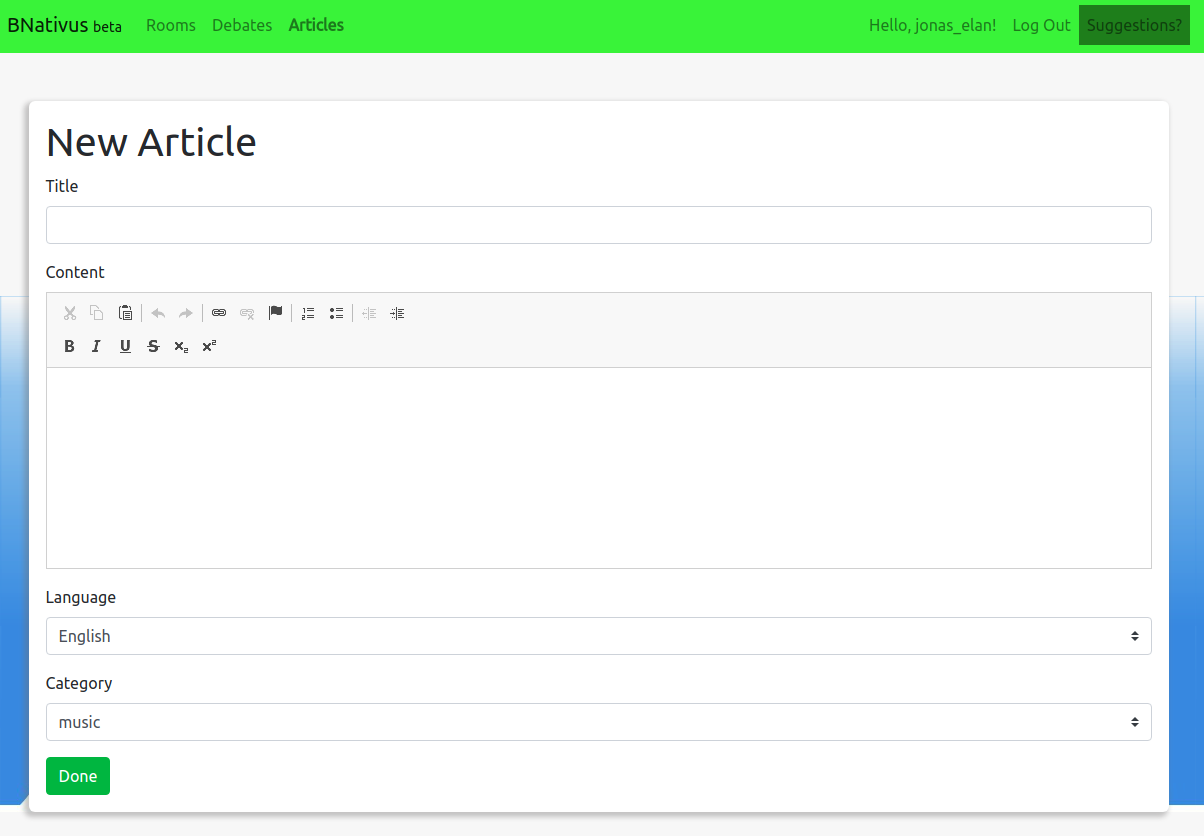
\includegraphics[width=15cm, height=10cm]{src/imagens/criar-artigo.png}
      	\textsf{\caption{Tela de criação de artigos}}
      	\label{fig:FiguraTeste}
    \end{figure}    
        
    \begin{figure}[!htb]
    	\centering
      	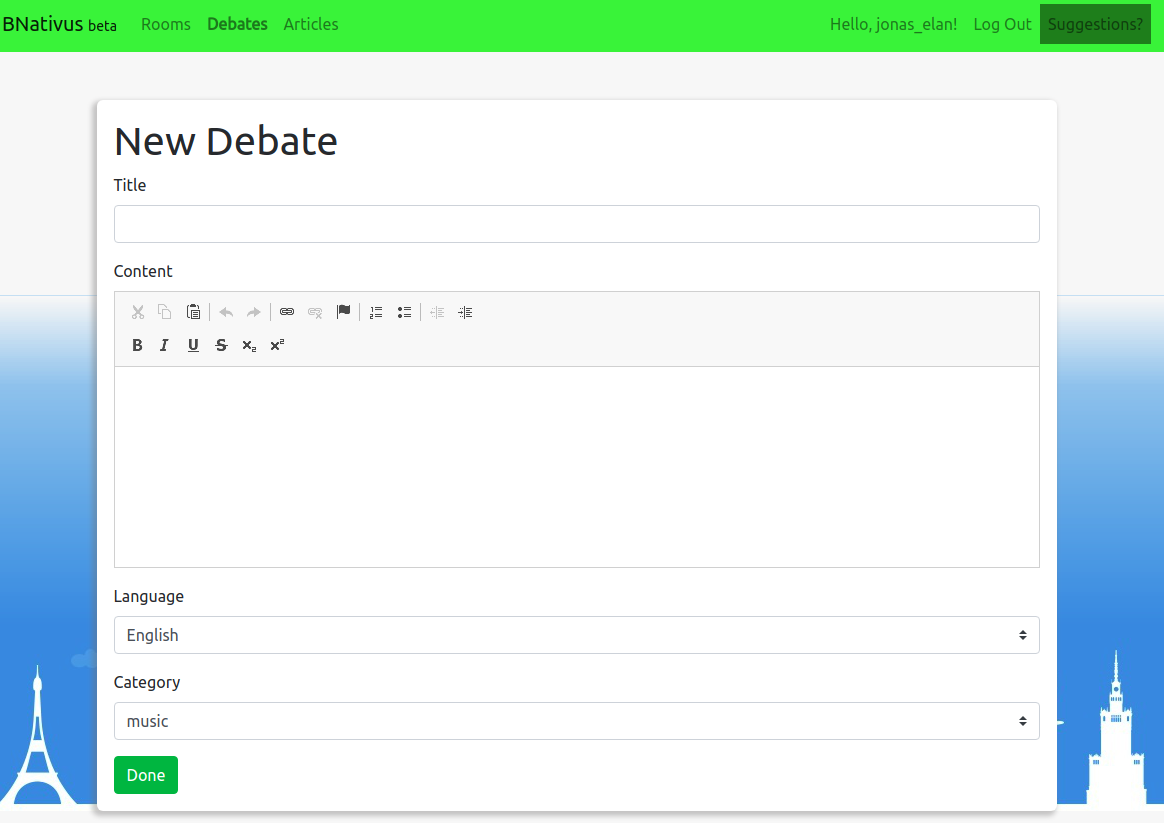
\includegraphics[width=15cm, height=10cm]{src/imagens/criar-debate.png}
      	\textsf{\caption{Tela de criação de debates}}
      	\label{fig:FiguraTeste}
    \end{figure}
    
    \newpage
    
    Nas figuras acima, é possível visualizar melhor o que constitui as postagens, e como as suas telas de cadastros são semelhantes. Elas possuem um título, a linguagem em que foi escrito o texto, e uma categoria, para que o usuário possa ter mais informações, antes mesmo que abra a postagem. Além disso, o campo conteúdo foi integrado a uma ferramenta de edição de texto. Ela possui o básico para se escrever textos, como negrito, copiar e colar, \textit{upload} de imagem, listagem de itens, dentre outras opções. Dessa forma, usuários que desejam utilizar essas funcionalidades terão maior liberdade no momento da escrita.

    \item Alterar idioma do site

    Quando se constrói um sistema, é primordial que desenvolva tudo pensando no usuário, pois é para ele que o software é feito. O BNativus seguiu essa filosofia, acreditando que seria importante possuir uma funcionalidade de alterar o idioma de todo a plataforma web, pois dessa forma, se torna mais maleável, visto que haverá acesso de diferentes pessoas, com diferentes línguas de estudo. Além disso, já está adaptado para o futuro, caso for acessado por estrangeiros que procuram estudar línguas também.
    
    O Ruby on Rails, já visando o quão problemático e complexo é a criação de plataformas multi-linguagens, possui suporte, desde suas versões mais antigas, a internacionalização, usando a API i18n (18 é o número de letras entre o I e o N na palavra \textit{internalization}). Para implementar, basta mapear todas as strings, e, manualmente, atribuir valores a cada uma delas. Elas são mapeadas por arquivos YAML que ficam localizados dentro da pasta config/locale, e cada um deles representa uma linguagem \citeonline{Rails}.
    
    \begin{figure}[!htb]
    	\centering
      	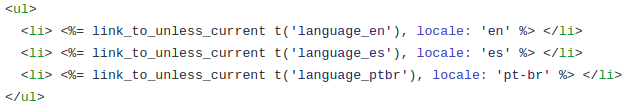
\includegraphics[width=16cm, height=3cm]{src/imagens/link_footer.png}
      	\textsf{\caption{Trecho em HTML dos links para alterar o idioma do sistema}}
      	\label{fig:FiguraTeste}
    \end{figure}
    
    \begin{figure}[!htb]
    	\centering
      	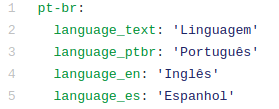
\includegraphics[width=8cm, height=3cm]{src/imagens/i18n_yaml.png}
      	\textsf{\caption{Trecho em YAML com a representação de como ficará o texto dos links em português}}
      	\label{fig:FiguraTeste}
    \end{figure}
    
    Os trechos de código mostrados acima são referentes ao rodapé da aplicação, que é visível em todas as páginas do sistema. Nessa seção há três botões (o código é mostrado na figura 16) que são responsáveis pela alteração da linguagem da plataforma. A figura 17 demonstra o texto dos links em português.
\end{enumerate}

\subsubsection{Segunda sprint}

    Com a parte mais importantes do sistema implementado, foram estabelecidas algumas novas funcionalidades para melhorar o que já foi feito, e adicionar mais segurança, que até o momento, estava totalmente aberta e sem autenticação. Até o momento do início da segunda sprint, não houveram grandes dificuldades, com um fluxo de desenvolvimento dentro do planejado, mas com algumas melhorias que já foram previstas e eram necessárias.

\begin{enumerate}
    \item Autenticação do usuário
    
    A autenticação é uma das vertentes mais importantes quando se trata de segurança. É através dela que é possível garantir que quem está usando o sistema, tendo acesso somente a suas informações, com os seus direitos que foram atribuídos. E como o BNativus foi planejado para ser acessado por diversas pessoas, é de suma importância garantir a elas que as informações pessoais não serão cedidas a alguém com más intenções.
    
    O Ruby on Rails não possui suporte nativo a autenticação. Para agilizar esse processo, que é bastante difundido, com muitos exemplos na internet, foi usado uma das bibliotecas mais populares no GitHub, o Devise. Sua instalação é simples, e já integra a aplicação pequenas mudanças, que facilitam o desenvolvimento, por exemplo métodos para verificar se o usuário está logado, internacionalização, geração de páginas padrões de login e registrar, envio de email (para casos como “esqueci minha senha” ou confirmar o cadastro do usuário). Tudo isso é facilmente configurado em um único arquivo, que contém diversas variáveis para configurar essas funcionalidades e outras.
    
    \begin{figure}[!htb]
    	\centering
      	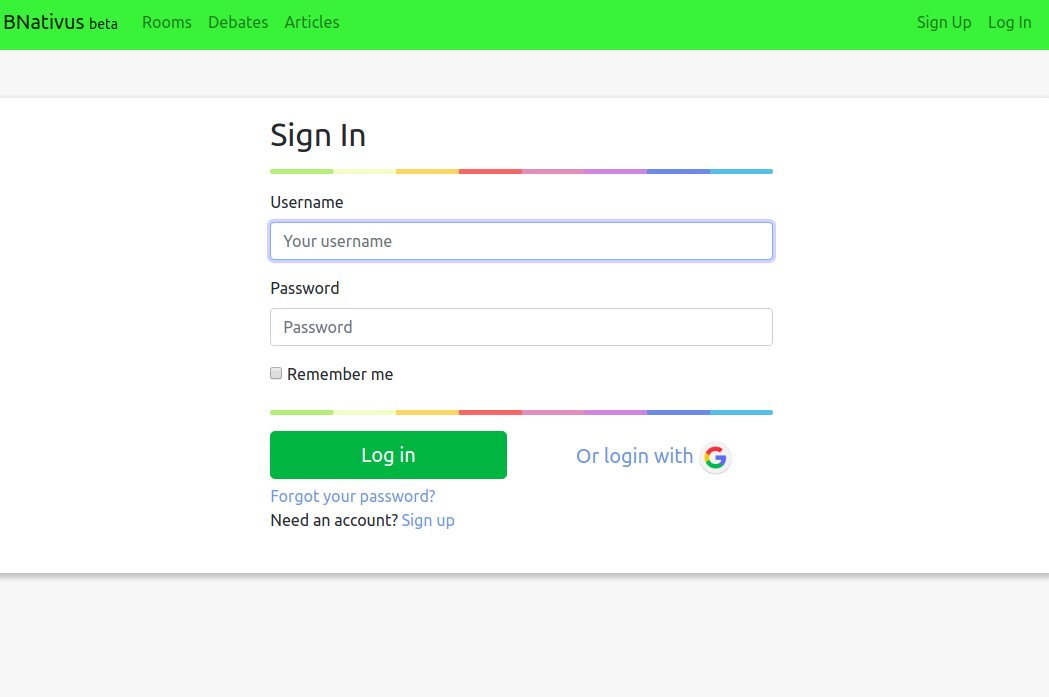
\includegraphics[width=14cm, height=8cm]{src/imagens/login.png}
      	\textsf{\caption{Tela de login}}
      	\label{fig:FiguraTeste}
    \end{figure}
    
    \begin{figure}[!htb]
    	\centering
      	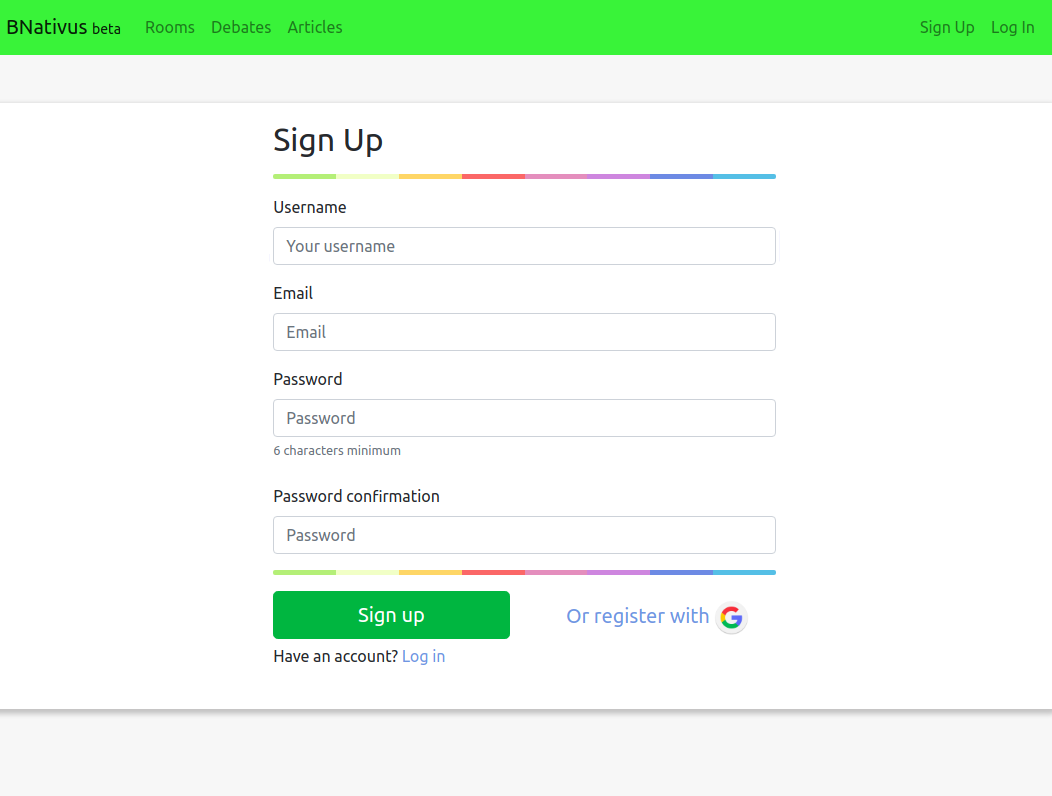
\includegraphics[width=14cm, height=10cm]{src/imagens/register.png}
      	\textsf{\caption{Tela de registro}}
      	\label{fig:FiguraTeste}
    \end{figure}
    
    \newpage
    
    Como é possível observar nas figuras, as duas telas são semelhantes com a única diferença que ao se registrar (Sign up), é necessário informar mais alguns dados básicos suficientes para criar sua conta e já começar a utilizar. É possível alterar esses dados ou até mesmo adicionar mais alguns, como data de nascimento ou foto. Frisando que a estrutura da página utilizado aqui foi reaproveitado do Devise, que inclusive criou controladores e modelos, para gerenciar toda a lógica um pouco complexa que há por trás da autenticação.

    Outra coisa notada é que existe a opção de se logar da forma tradicional, informando email e senha, ou utilizando a API do Google. Essa última é maneira mais simples de se conectar, pois basta um simples clique no BNativus e se conectar ao Google, liberando as permissões de acesso, para que o BNativus possa acessar as informações da conta Google. A autenticação dessa forma se mostra mais prática. Foi priorizado o uso do Google para esse tipo de funcionalidade, uma vez que a maioria dos recursos do BNativus utiliza o Hangout, outro serviço da empresa de tecnologia. Desta forma, se o usuário optar por se conectar através do Google, ele já estará logado e pronto para criar uma sala de conversa. Foi realizado toda a implementação com a API do Facebook também, no entanto, até o momento da construção do BNativus, a segurança da API para requisições HTTP, com a autorização OAuth\footnote{OAuth 2.0 é um protocolo para autorização e é focado em desenvolvimento simples enquanto disponibilização autorizaçao para serviços web (https://oauth.net/2/)}, foi bloqueada. Essa foi uma medida de segurança, pois é permitindo apenas requisições HTTPS. Requisições desse tipo não podem ser feitas no ambiente disponibilizado no desenvolvimento do BNativus. Portanto, relacionar o Facebook ao projeto ficou em segundo plano. No futuro, quando a aplicação estivesse em produção, será possível testar a autenticação através do Facebook com sucesso\footnote{https://developers.facebook.com/blog/post/2017/12/18/strict-uri-matching/}.


    \item Cadastrar línguas nativa e de estudo

    Como o BNativus se trata de um sistema de estudo de línguas, é de suma importância que os usuários informem o idioma que já domina, ou que dominam, tal como os idiomas que estão sendo estudados. Foi pensando em como fazer com que o usuário informasse esses dados, sem perder muito tempo na página de cadastro, ou seja, sendo mais direto e quebrando em partes o processo de cadastramento ao BNativus, caso não houvesse essa preocupação, o usuário poderia não se sentir confortável no seu primeiro acesso, pois teria que informar diversos dados.
    
    A solução encontrada foi criar uma camada adicional entre a página de cadastro e a página inicial. Essa camada é uma nova página, que é mostrada ao usuário somente no primeiro acesso, pedindo informações da língua, ou línguas, que domina e a que está estudando. A página pode ser observada na figura 20:
    
    \newpage
    
    \begin{figure}[!htb]
    	\centering
      	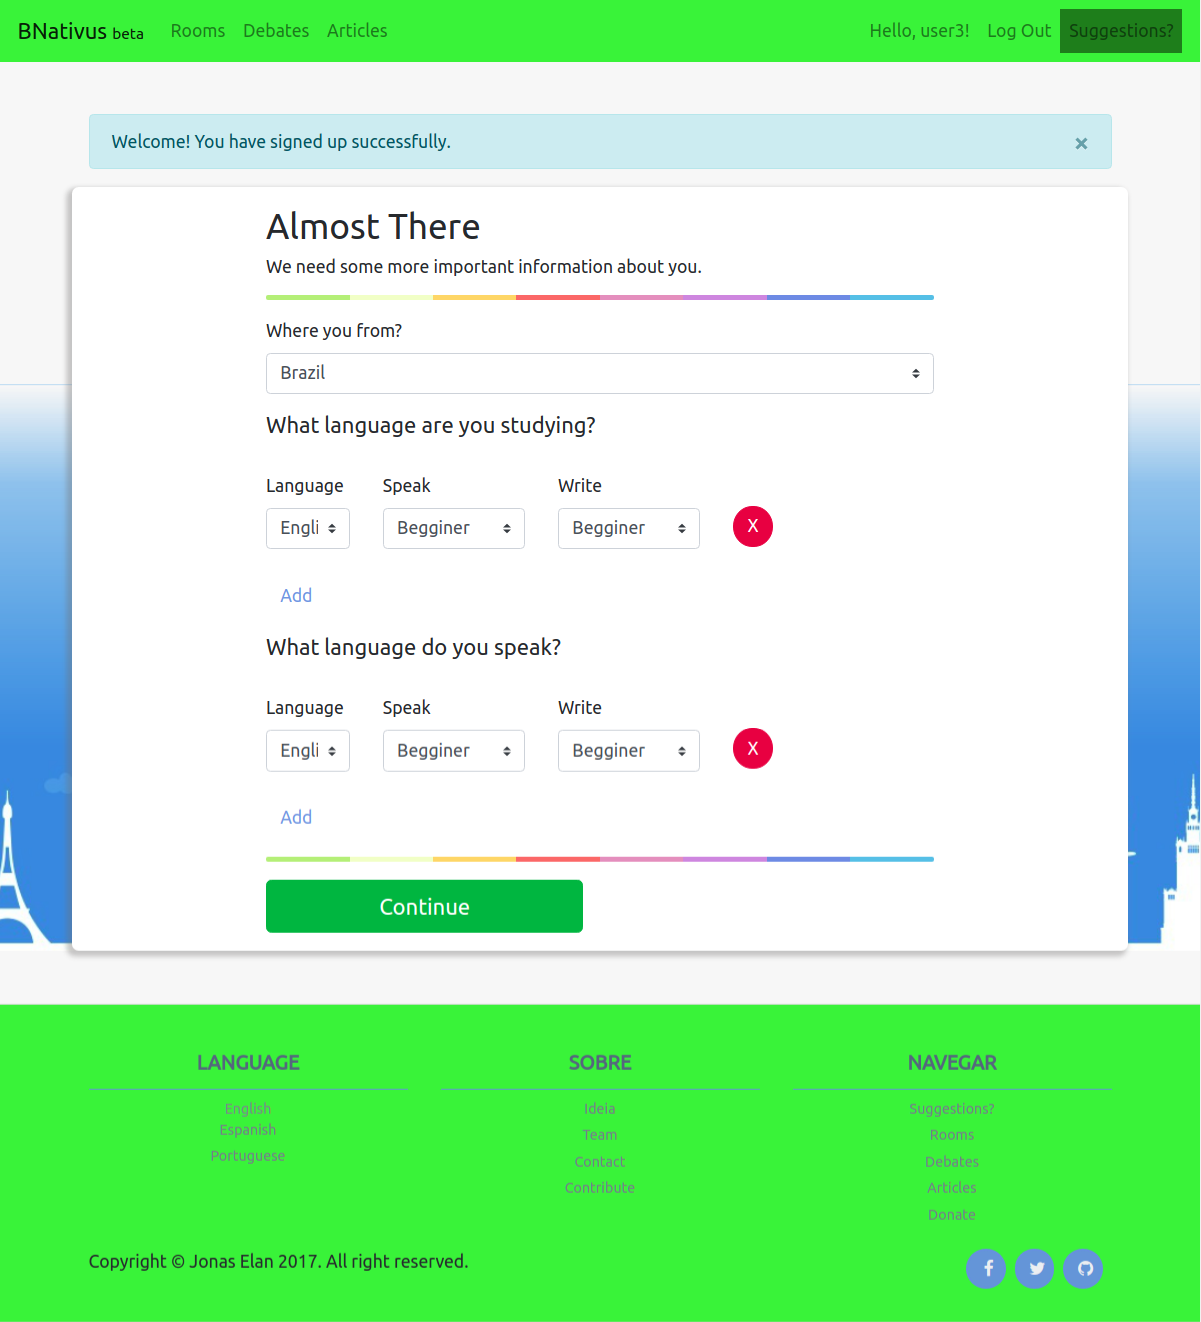
\includegraphics[width=15cm, height=17cm]{src/imagens/more_infos.png}
      	\textsf{\caption{Tela aonde o usuário informa as línguas de estudo e as que já domina}}
      	\label{fig:FiguraTeste}
    \end{figure}
    
    Para adicionar novos idiomas, basta clicar em \textit{Add}, e para remover, clicar no botão vermelho específico. Outra coisa a ser notada são as mensagens \textit{flash}, que são mensagens mostradas ao usuário após realizar alguma ação. No caso da figura 20, é mostrado uma mensagem de boas-vindas, após o usuário se cadastrar.

    \item Votar em debate e artigo

    O BNativus foi idealizado para criar um ambiente totalmente colaborativo entre a comunidade, portanto é necessário manter uma boa forma de interação entre os usuários. Na seção de artigos e debates, além de comentários, foi adicionado a opção de votos. Dessa maneira, outras pessoas podem se expressar de uma forma diferente, disponibilizando o \textit{feedback}, que é necessário para que o autor saiba se o que escreveu é relevante para mais pessoas, que não necessariamente precisam escrever algum comentário para transmitir essa informação.
    
    \begin{figure}[!htb]
    	\centering
      	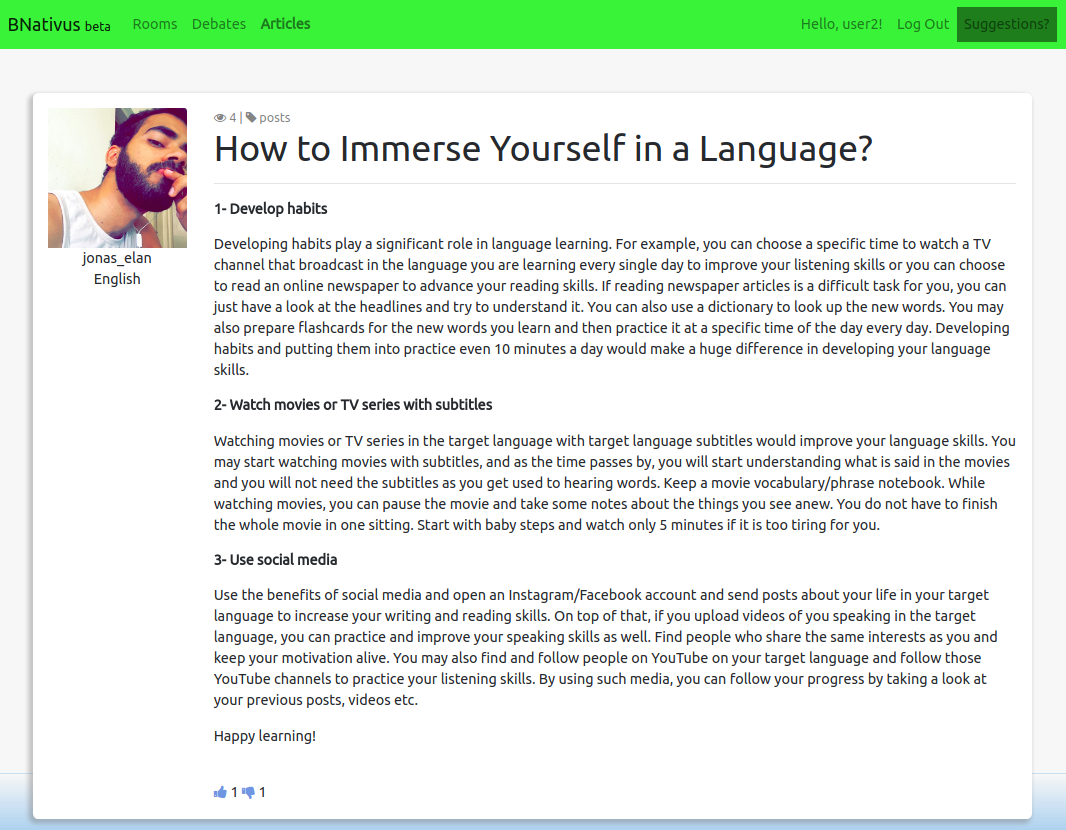
\includegraphics[width=16cm, height=12cm]{src/imagens/text_article.png}
      	\textsf{\caption{Exemplo de artigo}}
      	\label{fig:FiguraTeste}
    \end{figure}
    
    A figura 21 mostra um exemplo de como é a página de visualização de artigo. A página de debates é praticamente igual. É possível notar, na parte inferior na imagem os botões de votação, representados pelo polegar para cima e outro para baixo, representando o voto positivo e negativo, respectivamente. Nessa imagem é possível perceber também onde ficam dispostos o autor, a linguagem, a categoria e o número de visualizações. Algumas dessas informações são úteis também para filtros durante a listagens de postagens. Dessa forma, encontrar postagens se torna mais fácil.

    \item Criar página pública e inicial

    O conjunto dessas funcionalidades citadas até então já engloba praticamente todo o escopo planejado no sistema. No entanto, é importante tornar as salas, debates e artigos de fácil acesso, em um local central (não somente no cabeçalho, que está basicamente em todas as páginas). Em outras palavras, era preciso criar uma página inicial do usuário, onde ele poderia ver, dividido por seção, as postagens e salas de conversa mais recentemente criados, além de poder acessar as criadas por ele mesmo anteriormente.

    \begin{figure}[!htb]
    	\centering
      	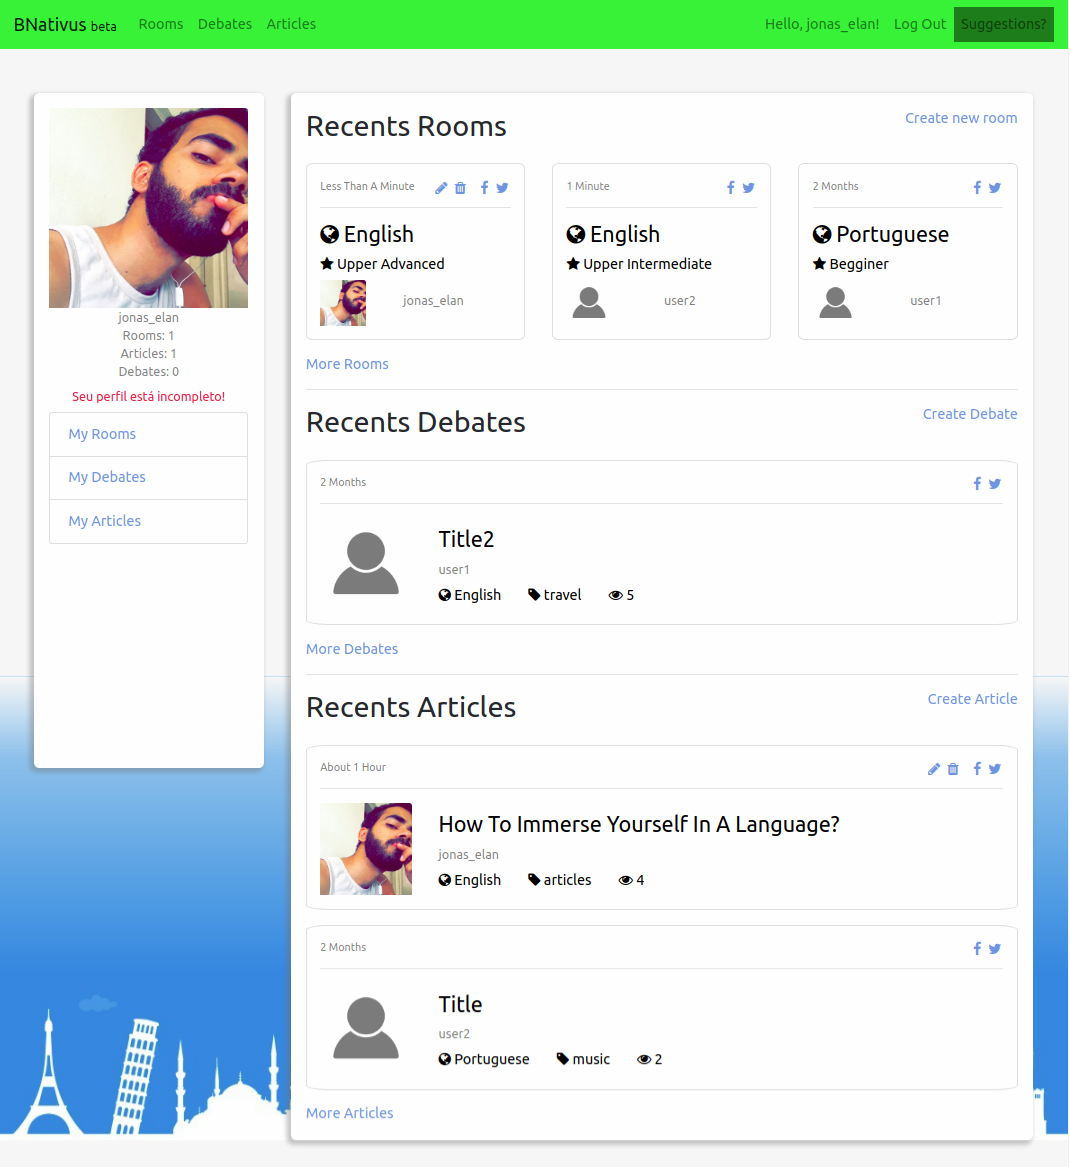
\includegraphics[scale=0.40]{src/imagens/home.png}
      	\textsf{\caption{Tele inicial}}
      	\label{fig:FiguraTeste}
    \end{figure}
    
    A imagem acima retrata como ficou a página. Ela foi dividida em duas partes: área central, que contém os cartões de debates, artigos e salas de conversa e a outra é o menu lateral, que contém informações pessoais, como o \textit{nickname}, foto de perfil, a quantidade de recursos criados e etc. 

	Pensando na praticidade e organização, foi decidido que debates, artigos e salas de conversas seriam disposto, dentro de todo o sistema, como cartões. Em cada deles, são colocadas algumas informações básicas importantes, como quem o criou, qual linguagem ele foi criado e em que horário foi criado, além de informações específicas de cada recurso (categoria para postagens e o nível na língua para salas, por exemplo). Ainda observando a imagem, é notado que o usuário autenticado consegue gerenciar os recursos de sua autoria através dos cartões. Na parte superior direita há um ícone para editar (lápis) e excluir (lixeira).

    \begin{figure}[!htb]
    	\centering
      	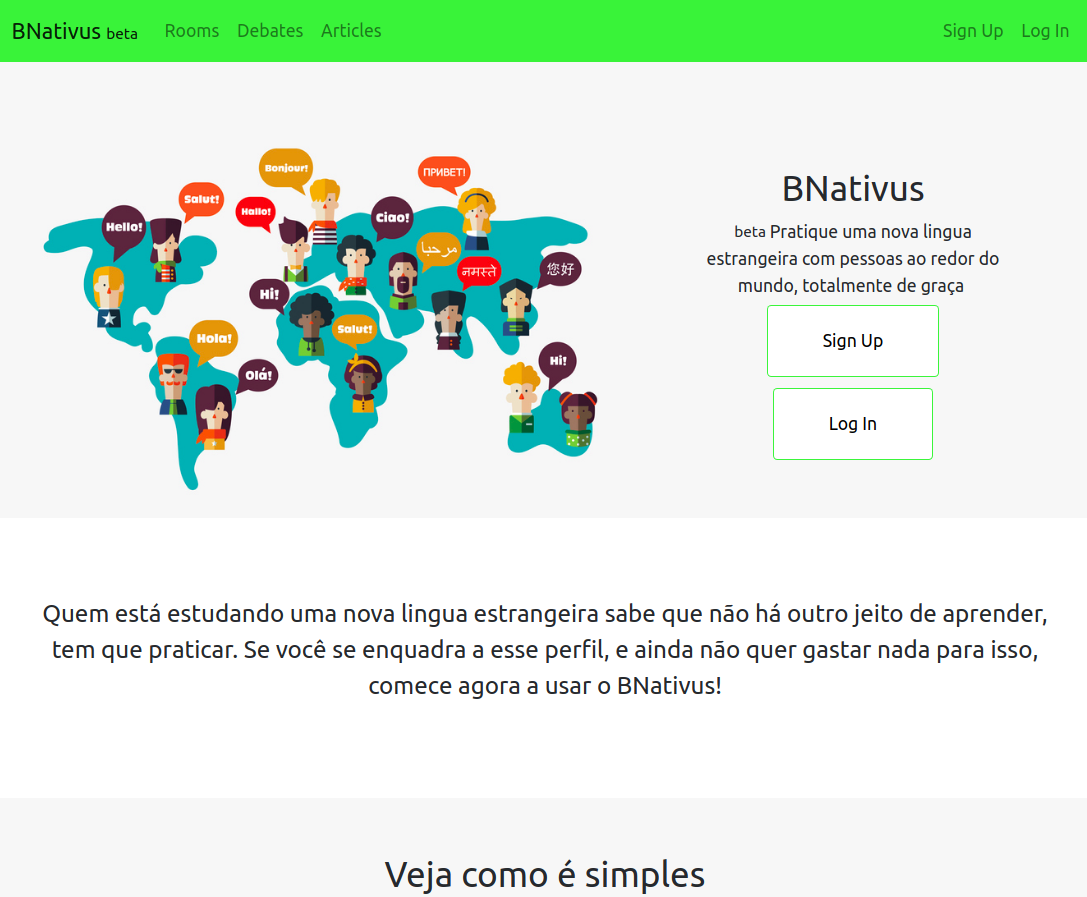
\includegraphics[scale=0.4]{src/imagens/public_home.png}
      	\textsf{\caption{Parte da tela pública com informações sobre a aplicação}}
      	\label{fig:FiguraTeste}
    \end{figure}
    
    Há ainda a página pública, que todos possuem acesso, que explica como o BNativus funciona. O cuidado no estilo presente nesta página foi maior, pois se ela fosse chamativa e ao mesmo tempo simples, sem muitas informações, chamaria a atenção das pessoas, aumentando as chances de se tornarem usuárias de fato. Ela pode ser observada na figura 23.
\end{enumerate}

\subsubsection{Terceira sprint}

Nessa última fase, que durou todo o mês de dezembro de 2017,  foi adicionado algumas pequenas funcionalidades sutis, mas importantes para o sistema. Elas serão explicadas melhor ao longo do desta seção.

\begin{enumerate}
    \item Comentar debate e artigo
    
    Nas duas formas de postagens abordadas no sistema web aqui apresentado, é possível realizar comentários. O principal intuito com essa funcionalidade é adicionar uma forma extra de praticar escrita ao mesmo tempo que melhora ainda mais a interações entre os usuários. O seu uso é mais direcionado aos debates, uma vez que para que esse tipo de conversa possa acontecer, é preciso de duas ou mais pessoas. Portanto, ao criar um debate, a comunicação é realizada através dos comentários. A opção de comentário também está presente nos artigos, todavia, o diálogo previsto é menor.

	Foi iniciado o seu desenvolvimento manualmente, da mesma forma que foi feito com as salas, por exemplo, com a criação de modelos, controladores e páginas específicas. Porém, logo foi observado que este fragmento do sistema não seria tão simples, e exigiria um tempo maior de desenvolvimento. Por isso, foi buscado outras formas de implementação. Dentre os pesquisados, e o que melhor se enquadrou as necessidades, foi o Disqus\footnote{https://disqus.com/}, sistema web focado em manter o engajamento de pessoas através de comentários.

    \newpage
    
    \begin{figure}[!htb]
    	\centering
      	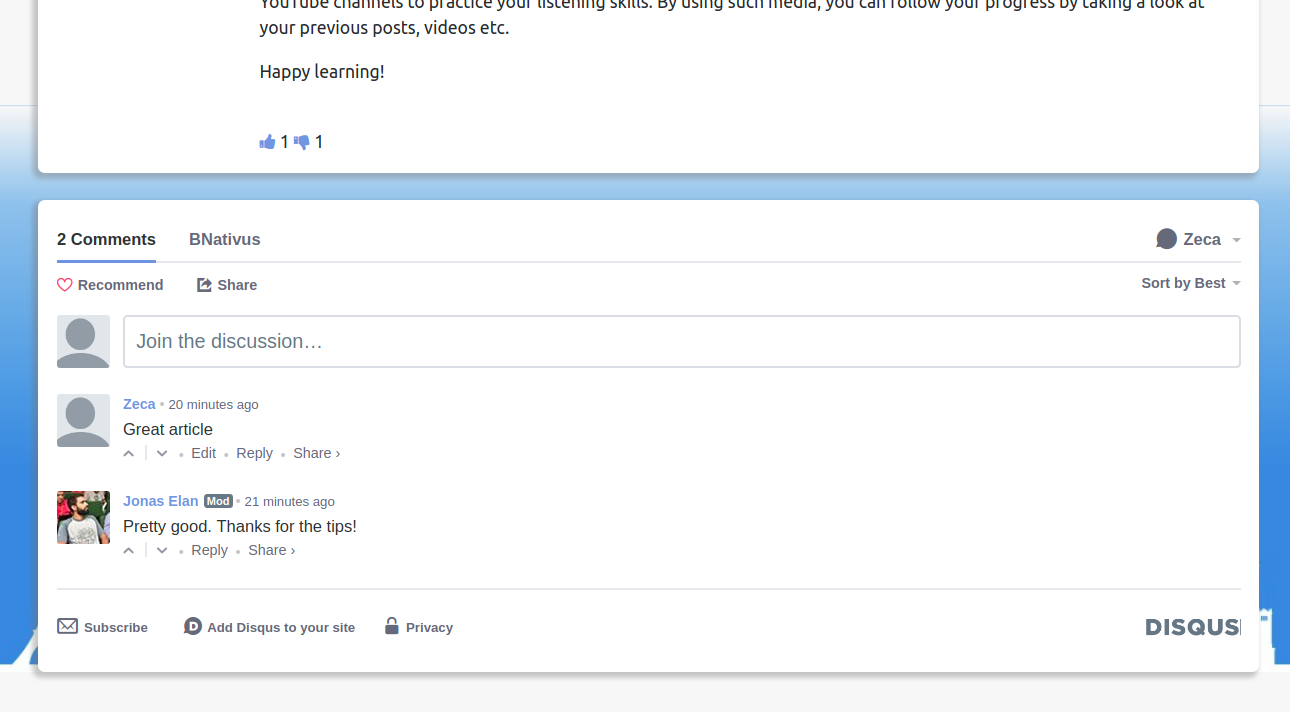
\includegraphics[scale=0.34]{src/imagens/disqus.png}
      	\textsf{\caption{Comentário dentro da plataforma BNativus}}
      	\label{fig:FiguraTeste}
    \end{figure}

    Terceirizar essa parte do BNativus ao Disqus poupou muito tempo, uma vez que ele é bem completo e de integração fácil (apenas adicionar um script Javascript à página), necessitando apenas de uma conta no serviço, que pode ser feito através do Facebook, Google ou Twitter. Boa parte de suas funcionalidades são gratuitas, como comentários, resposta a comentários, compartilhamento, ordenação e etc. A conta criada para a integração ao BNativus dispõe de uma seção administradora, onde é possível monitorar o que é feito, e onde há maior movimentação dentro do sistema, além de permitir ou não que certos tipos de comentários sejam aceitos dentro da plataforma.  
    
    \newpage 

    \begin{figure}[!htb]
    	\centering
      	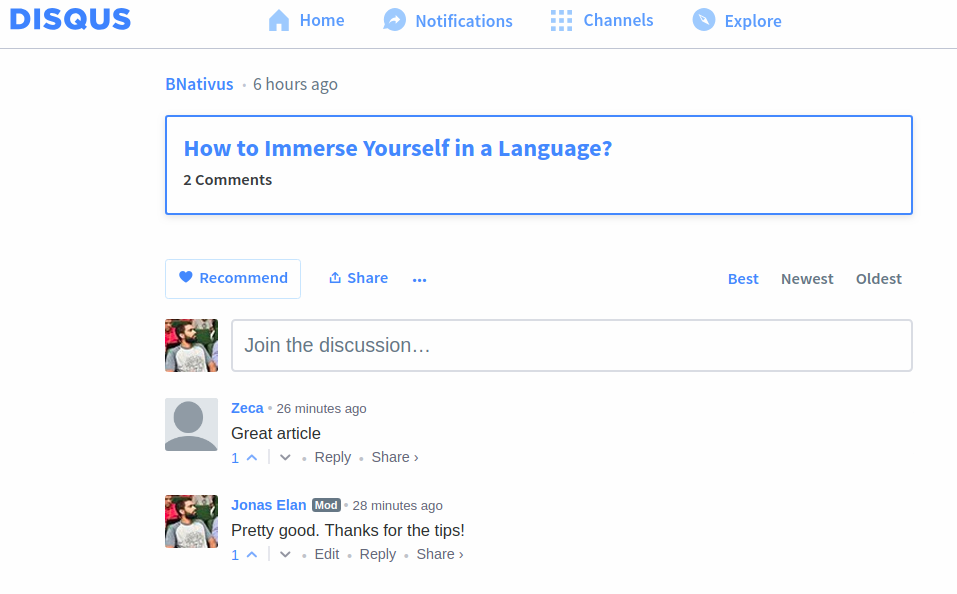
\includegraphics[scale=0.4]{src/imagens/disqus2.png}
      	\textsf{\caption{Comentário dentro da plataforma Disqus}}
      	\label{fig:FiguraTeste}
    \end{figure}
    
    \item Editar perfil
    
    Como já foi citado anteriormente, com poucas informações já é possível começar a utilizar o sistema, no entanto há outros dados que são interessantes serem preenchidos, pois complementando o perfil, outras pessoas podem conhecer um pouco melhor o outro, caso não consigam se comunicar corretamente dentro dos recursos que o sistema disponibiliza, ou até antes mesmo de começar a comunicação. Para que seja possível visualizar e editar os dados pessoais, foi criado uma página específica, que podem ser acessadas através do botão localizado no canto direito do cabeçalho, no qual mostra o nome de usuário.
    
    Para lembrar aos usuários de completar o seu cadastro, no menu lateral, localizada na página inicial, há uma mensagem, informando que o perfil está incompleto, e que é recomendável informar os demais dados. Ele pode ser observado na 22.
    
    \newpage
    
    \begin{figure}[!ht]
    	\centering
      	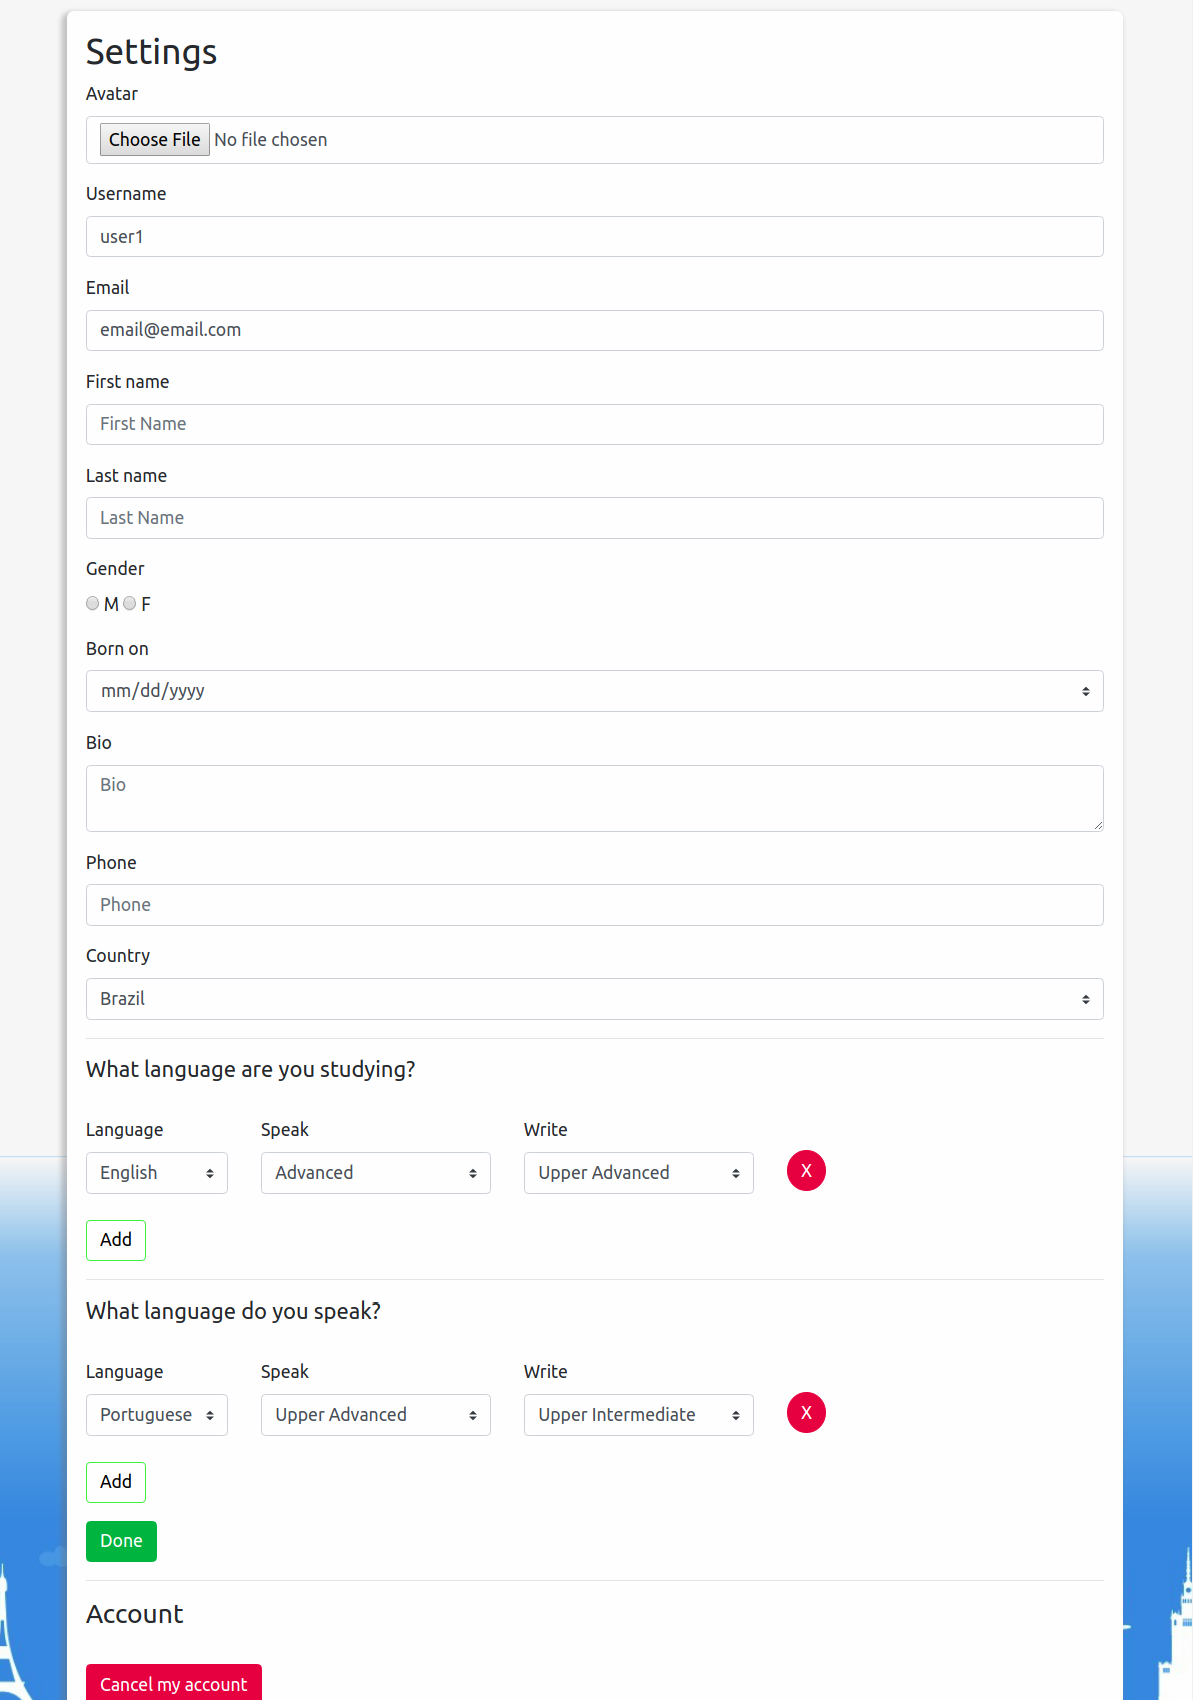
\includegraphics[scale=0.38]{src/imagens/edit.png}
      	\textsf{\caption{Tela de edição de perfil}}
      	\label{fig:FiguraTeste}
    \end{figure}
    
     \newpage
    
     \item Compartilhamento de salas, debates e artigos
    
	Como o BNativus é um sistema que ainda está evoluindo, e provavelmente não vai possuir tantos acessos no período inicial de sua implantação, foi pensando em uma forma de fazer com que os usuários, que já o utilizam, pudessem convidar outros, com os mesmos objetivos de praticar novas línguas. Uma forma simples de fazer isso é integrar mais uma vez redes sociais a aplicação.

	Em cada cartão há, no canto superior direito, dois botões, uma para compartilhar no Facebook e outro para o Twitter. Dessa forma, novas pessoas vão conhecer a plataforma, mesmo que não haja o engajamento de outras. 


    \begin{figure}[!htb]
    	\centering
      	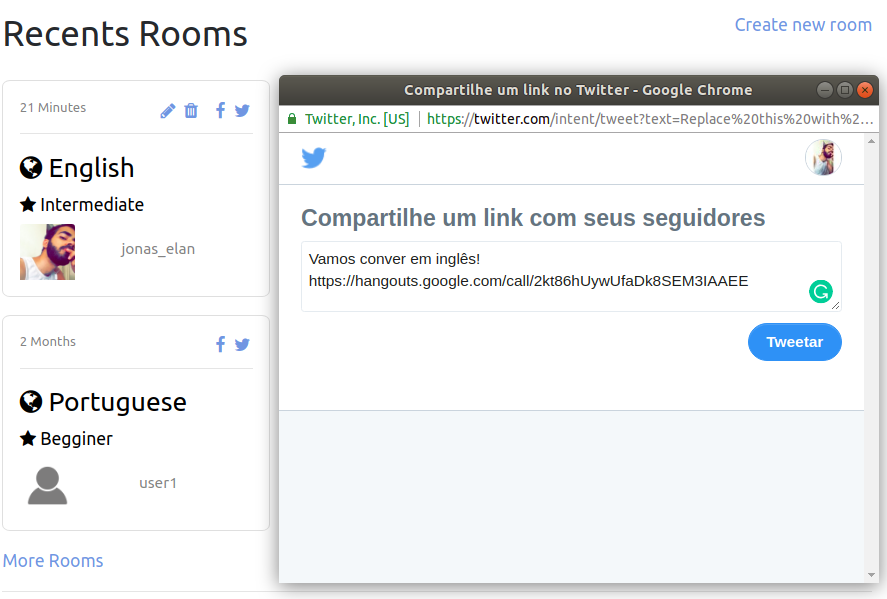
\includegraphics[scale=0.4]{src/imagens/twitter.png}
      	\textsf{\caption{Compartilhar para o Twitter}}
      	\label{fig:FiguraTeste}
    \end{figure}
    
    \newpage
    
    \begin{figure}[!htb]
    	\centering
      	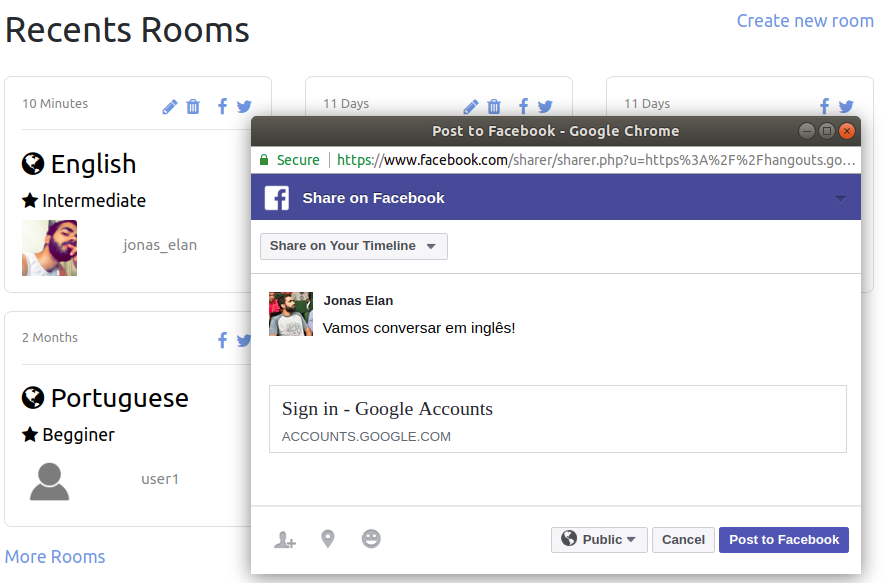
\includegraphics[scale=0.4]{src/imagens/fb.png}
      	\textsf{\caption{Compartilhar para o Facebook}}
      	\label{fig:FiguraTeste}
    \end{figure}

\end{enumerate}

\subsection{Fluxo de desenvolvimento}

Nos itens acima foram explicados as tarefas que foram estabelecidas, com alguns detalhes mais técnicos, tal como sua divisão em sprints e a organização planejada. Esta seção será reservada a explicar mais explicitamente como foi todo o fluxo de desenvolvimento feito em praticamente todas essas tarefas. 

O desenvolvimento do BNativus seguiu a ideia do TDD, com já foi explicado na fundamentação teórica, portanto todas as tarefas, antes de começarem a ser codificadas de fato, tinha os seus testes unitários criados. Após ter certeza que o teste falhou, é que se seguia para o desenvolvimento da funcionalidade. Quando rodar o teste novamente, o sinal positivo deve ser mostrado, e da mesma forma com as próximas funcionalidades. Com isso feito, foi necessário estabelecer alguma ferramenta de entrega contínua, que executasse esses testes em uma \textit{pipeline}, e se todos os testes passarem, a aplicação já ser implantada (colocada em produção).

Há diversas ferramentas no mercado que disponibilizam máquinas na nuvem que clonam a aplicação e os testes são executados nesse ambiente. Durante a pesquisa de qual usar, foi cogitado o Jenkins, CicleCI e o Travis. No fim, o Travis foi escolhido por sua facilidade de uso e integração com o GitHub, que é aonde o código da aplicação aqui descrita está armazenado e versionado. As demais opções se mostraram mais completas, mas também complexas, voltadas para sistemas maiores. Após integrar o GitHub com o Travis, todo o commit feito para a \textit{branch master}  e \textit{pull requests}, faz com que os testes unitários sejam executados.

\begin{figure}[!htb]
	\centering
  	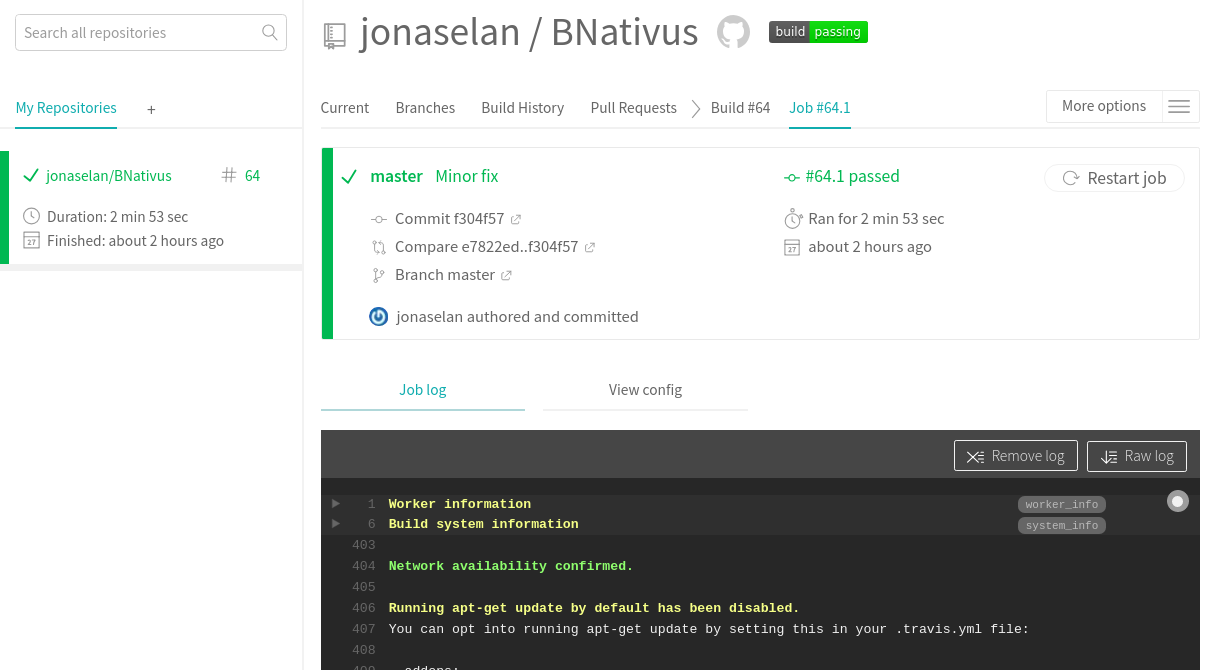
\includegraphics[scale=0.4]{src/imagens/travis.png}
  	\textsf{\caption{Dashboard dentro da plataforma Travis}}
  	\label{fig:FiguraTeste}
\end{figure}

\begin{figure}[!htb]
	\centering
  	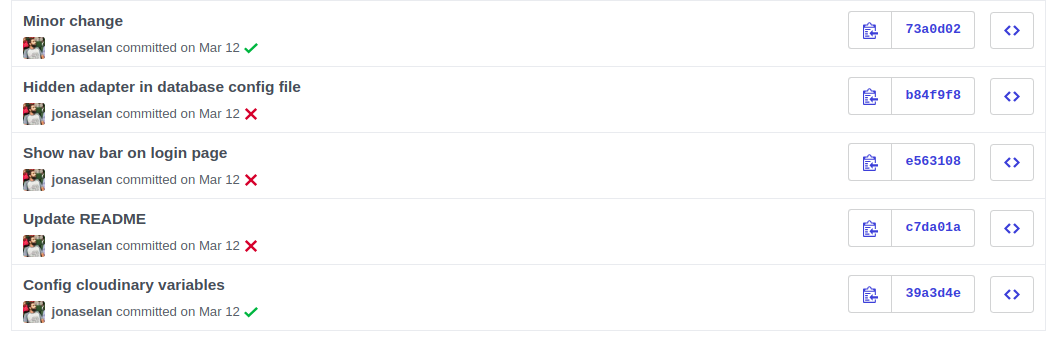
\includegraphics[scale=0.4]{src/imagens/github.png}
  	\textsf{\caption{Commits que passaram pela \textit{pipeline} de testes executadas pelo Travis}}
  	\label{fig:FiguraTeste}
\end{figure}
 
 O Travis disponibiliza gratuitamente uma máquina para executar os testes. Na figura 29 é demonstrado parte do painel de controle do Travis, com informações básicas sobre o commit, como tempo de execução, qual commit foi feito, para qual \textit{branch} e etc. Informações mais detalhadas são imprimidas em um terminal. Após executar todos os testes, no GitHub é mostrado um ícone ao lado das mensagens do commit, como pode ser observado na figura 30, informando se algum teste falhou, ou seja, se alguma modificação feita em um commit em específico interferir em outra parte do sistema, que já estava funcionando, o desenvolvedor é logo alertado e pode analisar melhor o que pode ter acontecido.

O Travis esteve presente durante praticamente todo desenvolvimento do sistema. Auxiliou de forma considerável, apesar de ter sido usado mais como uma forma de estudar e entender como funciona uma ferramenta de entrega contínua. Como foi idealizado utilizar os serviços da AWS para colocar a aplicação em produção, seria mais viável fazer uso da própria ferramenta de entrega contínua da Amazon, o CodePipeline, integrado com outros serviços de notificação, por exemplo. No próximo ponto, será discutido o porquê de não ter usado essa abordagem.

 
 